\documentclass[11pt]{article}
\usepackage[utf8]{inputenc}
\usepackage[T1]{fontenc}
\usepackage{amsmath,amssymb,amsthm,mathtools}
\usepackage{libertinus-otf}
\usepackage[margin=1in]{geometry}
\usepackage{graphicx,booktabs,array,longtable}
\usepackage{placeins}
\usepackage{microtype}
\usepackage[round,authoryear]{natbib}
\usepackage[hidelinks]{hyperref}
\usepackage{enumitem}
\setlist{itemsep=3pt,topsep=5pt}
\setlength{\emergencystretch}{2em}
\allowdisplaybreaks[2]
\numberwithin{equation}{section}
\newtheorem{theorem}{Theorem}[section]
\newtheorem{proposition}[theorem]{Proposition}
\newtheorem{corollary}[theorem]{Corollary}
\newtheorem{lemma}[theorem]{Lemma}
\theoremstyle{remark}
\newtheorem{remark}[theorem]{Remark}
\newcommand{\E}{\mathbb E}
\newcommand{\R}{\mathbb R}
\newcommand{\Q}{Q}
\newcommand{\cV}{\mathcal V}
\newcommand{\F}{\mathcal F}
\newcommand{\ind}{\mathbf 1}
\newcommand{\dd}{\,\mathrm d}
\DeclareMathOperator{\Var}{Var}
\DeclareMathOperator{\Cov}{Cov}
\DeclareMathOperator{\rank}{rank}
\DeclareMathOperator{\row}{row}
\DeclareMathOperator{\diag}{diag}
\newcommand{\pos}[1]{(#1)^+}
\hypersetup{pdftitle={What options reveal about policy-meeting risk}}
\title{What options reveal about policy-meeting risk:\\ identification and factor-model restrictions}
\date{September 27, 2026}
\begin{document}
\maketitle
\begin{abstract}
We characterize the meeting-risk allocations that derivative prices distinguish and the restrictions that factor specifications impose. In a Gaussian rate model, fixed post-cutoff cash claims, including American exercise, depend on earlier meeting and continuous variance only through their total; later-accruing futures retain one additional time-weighted moment. We give an exact calendar criterion for separating meeting risk from deterministic background volatility, and sharp conditional bounds from premium intervals. For scheduled-rate factor models, we characterize all variance vectors attainable under arbitrary deterministic scale recalibration and derive their exact support under square-root stochastic volatility, including the random drift and leverage terms. The published three-factor specifications of \citet{brace2024sofr} imply different active support dimensions. In 555 SOFR option chains on 78 dates, a smile fit reduces the median maximum strike error to 0.161 bp, but meeting-risk lower bounds remain sensitive to background assumptions. A loading with a free long-end level improves three-year-midcurve predictions. A discrete-outcome example quantifies the limits of an additive ATM-variance interpretation.
\end{abstract}
\noindent\textbf{Keywords:} SOFR options; scheduled policy meetings; identification; calibration; background volatility; partial identification.

\section{Introduction}
A calibrated SOFR model can assign a variance to every future policy meeting. Which of those numbers are determined by derivative prices, and which are selected by the model? This question has two parts. Prices may fail to distinguish different allocations of meeting risk. Conversely, a chosen factor specification may rule out allocations that the prices would permit. We characterize both restrictions, then examine how much of the distinction can be measured in public option settlements.

The first result is an exact price-equivalence statement. In a Gaussian rate model with scheduled jumps and deterministic continuous volatility, suppose a family of cash claims observes the forward curve only after a group of meetings. The time-zero value of every fixed cash payoff in that family depends on the earlier meeting and continuous variances only through their total. The statement includes American cash exercise, even when exercise decisions may use the full earlier history. Futures accruing after the group retain one additional quantity: their first time-weighted variance moment. Consequently, with three or more earlier meetings, even complete strike surfaces and these futures generally leave a continuum of indistinguishable allocations. With no continuous volatility and a zero initial curve, three equally spaced dates with variances $(200,300,200)$ and $(300,100,300)$ bp$^2$ give the same prices throughout the stated contract family. The middle meeting's standard deviation nevertheless changes from $17.3$ to $10$ bp.

The second result determines restrictions imposed by the factor model. For the scheduled-rate construction of \citet{brace2024sofr}, we characterize all event-variance vectors attainable under arbitrary deterministic scale recalibration. The set is a finitely generated cone: subdividing the scale intervals beyond the meeting dates adds no attainable vectors. When each factor gives all future meetings the same loading, its complete restrictions are consecutive-meeting variance inequalities controlled by the largest decay rate. We then derive the conditional event-variance map with square-root stochastic volatility, including the random Heath--Jarrow--Morton (HJM) drift and its covariance with the diffusion. We determine its support, the closed set of possible meeting-variance vectors, and hence all affine equalities and the covariance rank. Applied to the two published parameter specifications, the result gives support dimension at most two for the constant specification and at most three for the time-dependent specification. Factor count alone would not reveal this difference.

The third result concerns the observation calendar and price precision. In the Gaussian model with deterministic continuous volatility, an ideal cash option expiring before its futures accrual begins reveals accumulated meeting variance plus weighted continuous variance. We give an exact rank criterion for separating the two, allowing several background-variance parameters and known maturity-dependent loadings. Premium intervals then produce sharp conditional ranges for individual meetings and group totals. Two suitably chosen cash calls already identify the exact price parameters when the initial curve is known. The calendar criterion and optimization are elementary once the pricing map is established. Their role is to show when a reported meeting allocation is unique, how background flexibility changes that answer, and whether uniqueness survives realistic price precision.

These results lead to different tests. The first identifies an ambiguity that additional post-meeting strikes and exercise opportunities cannot remove. The second identifies restrictions that no scale calibration of a specified factor model can evade. The third determines which earlier expiries and background exposures supply the missing information. Sections~\ref{sec:prices}--\ref{sec:precision} develop the price and calendar results; Section~\ref{sec:restrictions} treats factor restrictions.

\subsection{Relation to existing work}
Extracting announcement risk from options is established practice. \citet{patell1979anticipated} documents option-implied variance changes around anticipated earnings releases. \citet{dubinsky2018option} separates scheduled earnings uncertainty from ordinary volatility using option prices; that article subsumes the earlier two-author working paper. \citet{leung2014accounting} studies scheduled earnings jumps and American exercise. For interest rates, \citet{beber2006effect} examines changes in option-implied Treasury-price distributions around macroeconomic announcements, while \citet{wright2020event} uses short-dated options to separate event-day and ordinary-day risk. None of these makes the principle of subtracting background variance a new contribution here.

The closest monetary-policy measurement study is \citet{bauer2021market}, which constructs a model-free short-rate uncertainty measure from Eurodollar futures and options and studies its changes around FOMC announcements. Its Appendix C explicitly identifies a difficulty with an ex ante meeting-variance estimator: successive quarterly contracts need not span the same meetings, while monthly expiries have less historical data and liquidity. Our criterion addresses the cross-sectional version of that problem. It states exactly which meeting cutoffs and background exposures identify a particular future allocation, allows several background cells and different underlying windows, and distinguishes rank from useful resolution at finite price precision. It is complementary to their event-study evidence about how uncertainty changes through time.

\citet{zhong2026spanning} studies identification when a flexible background option surface can absorb scheduled-event risk. Our stronger price-equivalence result concerns an entire post-cutoff family of interest-rate cash claims, including exercise decisions using earlier information, and explains why futures preserve one more variance moment than discounted cash claims. This differs from showing that one variance estimator or one implied-volatility surface decomposition is nonunique.

Policy-date term-structure models provide the economic and pricing setting. \citet{piazzesi2005bond} models the relation between Federal Reserve policy and bond yields; \citet{kim2014jumps} treats yield jumps at known dates. \citet{gellert2021short} distinguishes predictable short-rate steps from continuously evolving expectations in the forward curve. \citet{backwell2021expected} separates scheduled and unscheduled overnight-rate jumps and studies their effects on backward-looking contracts. The HJM drift restriction \citep{heath1992bond} and the general treatment of predictable discontinuities in \citet{fontana2018term,fontana2022term} supply the consistency framework. We use explicit specializations of that framework to study the inverse pricing problem.

For compounded overnight rates, \citet{lyashenko2019looking} develops a joint framework for forward- and backward-looking rates, \citet{heitfield2019inferring} studies term-rate inference from SOFR futures, and \citet{skov2021dynamic} derives dynamic SOFR futures models. \citet{itkin2024semi} treats SOFR-futures option valuation, including American exercise. These works explain why accrual, discounting, and exercise conventions belong in the pricing map. In our setting, cash discounting removes the first time-weighted variance moment from post-cutoff curve-payoff values, whereas futures expectations retain it. For futures-style exercise, the absence of an early-exercise premium is the established convex-submartingale result of \citet{lieu1990option,chen1993pricing}. We use it to determine exactly which meeting aggregates survive the change of contract convention.

The closest factor-model comparison is \citet{brace2024sofr}. That paper constructs scheduled short-rate dynamics with continuous fixed-maturity forward rates and calibrates stochastic volatility to futures and option smiles. Our contribution is to characterize restrictions implied by its loading and variance-state specification: those surviving arbitrary deterministic scale choices, and the exact stochastic support for fixed parameters. The square-root transition law itself is classical \citep{malham2008square}; the meeting-variance support and its active-column rank follow only after accounting for the full conditional variance kernel. This is also distinct from unspanned stochastic volatility in \citet{collindufresne2002bonds}, where volatility risk is not spanned by bonds within a model. Here we distinguish parameter allocations that give identical selected prices and determine the set of meeting variances permitted by a fixed specification.

Finally, sharp financial bounds from incomplete observations have a substantial optimization literature. \citet{bertsimas2002relation} obtains bounds on prices and moments by convex optimization; \citet{beiglbock2011model} develops model-independent bounds using martingale transport. Our bounds are conditional on the Gaussian observation map and the discount factors and means used in inversion. The linear program is standard. The specific content is the feasible set generated by meeting dates, background exposures, and premium intervals, together with the exact indistinguishable-allocation set for post-cutoff contracts.

\subsection{Data application and scope}
The application uses 4,100 selected strike observations in 555 CME SOFR option chains on 78 dates. The retained calendars never identify the complete meeting/background vector. A normal-mixture smile fit reduces the median maximum strike error to 0.161 bp, but the resulting ATM meeting-risk bounds remain sensitive to background flexibility. Same-expiry options on later underlying quarters add information about maturity loadings. A hump that returns to its initial level fails on three-year midcurves; allowing a free long-end level reduces their prediction error from 3.818 to 1.131 bp in standard deviation. Positive constant-background meeting bounds survive wider exercise and mean allowances, while flexible-background bounds still include zero. A discrete-meeting example shows why these ATM-proxy allocations need not equal actual outcome variances. A companion second-moment calculation instead exposes sensitivity to tail extrapolation. These findings favor compatible ranges and explicit model checks over a single calibrated meeting-volatility curve.

There are three separate mathematical settings. Sections~\ref{sec:prices}--\ref{sec:calendar} include an arbitrary deterministic initial curve and deterministic continuous volatility. Section~\ref{sec:aggregation} first proves aggregation in the pure-jump specialization and then extends it to the initial curve and continuous volatility; its explicit exercise formulas use the specialization. Section~\ref{sec:restrictions} studies the different scheduled-rate factor construction described above, conditional on the stated square-root solutions. The public-data calculation uses normal and mixture-based ATM proxies for listed American options, with separate numerical exercise and mean sensitivities. Their calibration ranges are conditional on the stated proxy observation maps. Section~\ref{sec:empirical} separates its pricing errors from its calendar restrictions, and Section~\ref{sec:uses} gives the resulting hedge and convexity applications.

\section{From a meeting model to observable option quantities}\label{sec:prices}
\subsection{Dates, rates, and units}
Time zero is the valuation date; time is measured in years. We use $t$ for observation time, $T$ for maturity, and $H$ for a fixed finite horizon containing all dates considered. The known future meeting dates are $0<T_1<\cdots<T_N<H$. At meeting $n$, a centred Gaussian surprise $X_n$ with variance $v_n\geq0$ is revealed. The $X_n$ are independent under the pricing measure $\Q$, the probability law used for valuation rather than a forecast of realized policy outcomes. They are also independent of a Brownian motion $W$, which represents information arriving between meetings. The information $\F_t$ available at time $t$ consists of the Brownian history and precisely those surprises whose dates have passed, with the usual augmentation. In particular, it contains no advance information about an unrevealed $X_n$.

The function $f_0(T)$ is the deterministic initial instantaneous forward rate for maturity $T$. The deterministic function $\sigma(s)$ is the volatility of the continuous component at time $s$. On a finite horizon, take $f_0$ bounded and piecewise continuous and $\sigma$ bounded and piecewise constant. For $0\leq t\leq T$, define
\begin{equation}\label{eq:curve}
f(t,T)=f_0(T)+\int_0^t\sigma(s)\,\dd W_s
 +\int_0^t\sigma(s)^2(T-s)\,\dd s
 +\sum_{T_i\leq t}\{X_i+v_i(T-T_i)\}.
\end{equation}
For clarity, $\alpha(t,T)$ is the forward drift, $\sigma(t,T)$ is the Brownian sensitivity, and $\xi_n(T)=f(T_n,T)-f(T_n-,T)$ is the announcement change. The present model is the specialization
\begin{equation}\label{eq:companion}
\alpha(t,T)=\sigma(t)^2(T-t),\qquad
\sigma(t,T)=\sigma(t),\qquad
\xi_n(T)=X_n+v_n(T-T_n).
\end{equation}
Here $X_n$ denotes the random level revealed at meeting $n$; the index labels separate announcements, rather than different maturity intervals within one announcement. The correction $v_n(T-T_n)$ is the affine correction required for a centred Gaussian level of variance $v_n$.

Each random surprise moves all remaining forward maturities by the same amount. The deterministic terms accompanying the diffusion and the surprises enforce bond-pricing consistency. They cannot be dropped without changing the pricing model.

The short rate is $r_t=f(t,t)$, the bank account is $B_t=\exp(\int_0^t r_s\,\dd s)$, and the zero-coupon bond price is $P(t,T)=\exp(-\int_t^T f(t,x)\,\dd x)$. Thus $P(0,T)=\exp(-\int_0^T f_0(x)\,\dd x)$ fits the initial curve exactly. Rates are decimals in formulas: ten basis points is $10^{-3}$, so a ten-basis-point meeting standard deviation corresponds to $v_i=10^{-6}$. Numerical tables rescale variances to squared basis points. A constant $\sigma=50$ bp per square-root year has variance rate $2{,}500$ bp$^2$ per year.

\begin{proposition}[Bond-pricing consistency]\label{prop:bond}
For each maturity $T$, the process $P(t,T)/B_t$, $0\leq t\leq T$, is a true martingale. Consequently $P(t,T)=\E[B_t/B_T\mid\F_t]$.
\end{proposition}
The proof in Appendix~\ref{app:pricing} writes the discounted bond as a product of Gaussian exponential martingales. This also specifies the stochastic assumptions behind the construction.

\subsection{The ideal futures payoff and its option}
Fix an accrual window $[a,b]$, with length $\delta=b-a>0$. The continuously compounded accumulation over this window and its futures expectation are
\begin{equation}\label{eq:futures}
R(a,b)=\exp\left(\int_a^b r_s\,\dd s\right),\qquad
G_t(a,b)=\E[R(a,b)\mid\F_t].
\end{equation}
The associated futures rate is $F_t=(G_t-1)/\delta$; this is a quoted rate, not the value of a futures position entered at time $t$. The distinction between $G$ and $F$ only changes the strike and scale. A European option expiring at $S\leq b$ with cash payoff $(G_S-K)^+$ has time-zero price
\begin{equation}\label{eq:cashcall}
C(S,K;a,b)=\E[B_S^{-1}(G_S-K)^+],\qquad K>0.
\end{equation}
A cash call on $F$ with rate strike $k$ has price $C(S,1+\delta k;a,b)/\delta$, provided $1+\delta k>0$.

These definitions specify the instruments in the theorems. A listed SOFR option is an option to enter a futures position, with exchange exercise, settlement, and daily-fixing conventions. Equation~\eqref{eq:cashcall} is a European cash contract. Section~\ref{sec:market} labels the approximation used when applying a simpler diagnostic to listed prices.

To state the pricing formula, let $\Phi$ and $\varphi$ denote the standard normal distribution and density. For a mean $m>0$ and a log variance $q>0$, write
\begin{equation}\label{eq:black}
\mathcal B(m,K,q)=m\Phi(d_+)-K\Phi(d_-),\qquad
 d_\pm=\frac{\log(m/K)}{\sqrt q}\pm\frac{\sqrt q}{2}.
\end{equation}
At $q=0$, define $\mathcal B(m,K,0)=(m-K)^+$. Thus $\mathcal B(m,K,q)=\E[(X-K)^+]$ when $\log X$ has mean $\log m-q/2$ and variance $q$. Here $m$ is the mean of $X$, while $q$ is the variance of its logarithm. The next proposition derives this distribution from the rate model.

\begin{proposition}[Price and information at one expiry]\label{prop:pricing}
For $s\geq0$, define the deterministic window weights
\begin{align}
w(s)&=(b-s)^+-(a-s)^+,\nonumber\\
d(s)&=\tfrac12\{((b-s)^+)^2-((a-s)^+)^2\},\qquad
h(s)=d(s)+\tfrac12 w(s)^2.\label{eq:weights}
\end{align}
Put $A_0=\int_a^b f_0(x)\,\dd x$ and
\begin{align}
p&=\sum_{i=1}^N h(T_i)v_i+\int_0^b\sigma(s)^2h(s)\,\dd s,\label{eq:p}\\
z&=\sum_{T_i\leq S}w(T_i)(S-T_i)v_i
       +\int_0^S\sigma(s)^2w(s)(S-s)\,\dd s,\label{eq:z}\\
q&=\sum_{T_i\leq S}w(T_i)^2v_i
       +\int_0^S\sigma(s)^2w(s)^2\,\dd s.\label{eq:q}
\end{align}
Then
\begin{equation}\label{eq:price}
G_0=e^{A_0+p},\qquad m=G_0e^{-z},\qquad
C(S,K;a,b)=P(0,S)\mathcal B(m,K,q).
\end{equation}
Knowing the entire function $K\mapsto C(S,K;a,b)$ for $K>0$ determines exactly the three price parameters $P(0,S)$, $m$, and $q$. Adding $G_0$ determines $z$. Adding the initial bond curve determines $p$.
\end{proposition}
The expiry-forward measure weights each outcome by its discount factor: for an expiry payoff $X$ with integrable discounted absolute value, its expectation is $\E^{S}[X]=\E[B_S^{-1}X]/P(0,S)$. Hence $m=\E^{S}[G_S]$ differs from the futures expectation $G_0=\E[G_S]$ because discounting changes the weights assigned to outcomes. This distinction is small numerically in some examples but essential to the identification argument.

A complete surface means prices at every positive strike with exact precision. It is a mathematical observation scheme. A few listed strikes do not automatically reveal all three parameters without error. In practice one fits or bounds them, keeping discount and mean uncertainty when material.

\begin{proposition}[Two fixed strikes suffice in the exact experiment]\label{prop:finitequotes}
Suppose the initial bond curve is known and $S\leq b$. Set $K_0=e^{A_0}$ and choose any fixed $K_1>K_0$. The two cash call prices at $K_0,K_1$ determine $(m,q)$ uniquely. Together with the underlying futures quote they determine $(p,z,q)$. This includes $q=0$.
\end{proposition}
The reason for choosing the first strike from the initial curve is that $m\geq K_0$ in this model. After scaling by $K_0$ and the known discount factor, the price at strike one fixes a curve of possible means and volatilities; the higher-strike price varies strictly along it. Appendix~\ref{app:finitecalendar} proves the assertion. It is an exact identification result, not a claim of a stable two-quote estimator. The chosen strikes may be illiquid or unlisted, and close price pairs can imply poorly determined parameters. Nevertheless, an entire strike surface is not required for the model's positive identification result.

\subsection{Why expiry intervals matter}
The particularly useful case is an option that expires before its underlying accrual begins: $S<a$. Every source of uncertainty revealed by $S$ then affects the entire window, so $w(s)=\delta$ for $s\leq S$. Define the accumulated rate variance
\begin{equation}\label{eq:Q}
\cV(S)=\sum_{T_i\leq S}v_i+\int_0^S\sigma(s)^2\,\dd s.
\end{equation}
Proposition~\ref{prop:pricing} gives
\begin{equation}\label{eq:Qz}
q=\delta^2 \cV(S),\qquad
\frac{z}{\delta}=\int_0^S \cV(x)\,\dd x.
\end{equation}
The normalized option log variance measures accumulated risk; the mean adjustment measures its time integral. Neither expression contains $f_0$. The whole option price still depends on the initial curve through $P(0,S)$ and $G_0$.

The variance difference between two expiries is especially transparent:
\begin{equation}\label{eq:increment}
\cV(S_2)-\cV(S_1)=\sum_{S_1<T_i\leq S_2}v_i
                         +\int_{S_1}^{S_2}\sigma(s)^2\,\dd s.
\end{equation}
It measures the meeting risks inside that interval plus the background variance accumulated over the same interval. It does not tell the two contributions apart by itself.

\section{Which meeting risks does the expiry calendar identify?}\label{sec:calendar}
\subsection{The observed panel}
Suppose the observed expiries are $0<S_1<\cdots<S_L$. Expiry $S_\ell$ may refer to its own accrual window $[a_\ell,b_\ell]$, but assume $S_\ell<a_\ell$ throughout. Divide its fitted log variance by $\delta_\ell^2$, where $\delta_\ell=b_\ell-a_\ell$, to obtain $\cV(S_\ell)$. In this section these quantities are observed exactly.

Represent the background variance rate by $n_b$ nonnegative parameters. Fix $0=c_0<c_1<\cdots<c_{n_b}$, with $c_{n_b}\geq S_L$, and set $\sigma(s)^2=u_j$ on $[c_{j-1},c_j)$, with $\sigma=0$ after $c_{n_b}$. The parameter vector is
\[
\theta=(v_1,\ldots,v_N,u_1,\ldots,u_{n_b})^\top\geq0.
\]
For an interval $J$, let $\mathfrak l_j(J)$ be the length of its intersection with $[c_{j-1},c_j)$. The observed vector $\boldsymbol{\cV}=(\cV(S_1),\ldots,\cV(S_L))^\top$ satisfies
\begin{equation}\label{eq:panel}
\boldsymbol{\cV}=\mathsf A\theta,\qquad
\mathsf A_{\ell i}=\ind_{\{T_i\leq S_\ell\}},\qquad
\mathsf A_{\ell,N+j}=\mathfrak l_j((0,S_\ell]).
\end{equation}
Thus calibration of these observations is a nonnegative linear inverse problem. The restriction $\sigma=0$ after $c_{n_b}$ completes the model outside the panel horizon; observations through $S_L$ provide no evidence for that tail restriction. The columns for meetings record whether each meeting has occurred by an expiry. The remaining columns record the exposure to each background-variance interval.

Set $S_0=0$ and call $(S_{\ell-1},S_\ell]$ expiry gap $\ell$. Let $E$ be the indices of gaps containing no meeting.

\begin{theorem}[Calendar criterion]\label{thm:rank}
The map $\theta\mapsto\mathsf A\theta$ is one-to-one on the set of nonnegative parameter vectors if and only if all three conditions hold:
\begin{enumerate}
\item every modelled meeting occurs by $S_L$;
\item each expiry gap contains at most one meeting;
\item the matrix $\Lambda_E=(\mathfrak l_j((S_{\ell-1},S_\ell]))_{\ell\in E,\,1\leq j\leq n_b}$ has rank $n_b$.
\end{enumerate}
Equivalently, $\rank\mathsf A=N+n_b$. If rank is deficient, every strictly positive parameter vector has a distinct strictly positive neighbour with the same variance panel.
\end{theorem}
The proof is row differencing. A meeting-free gap yields a linear equation involving only background variance. Once those equations determine the background, a gap containing one meeting determines that meeting's variance by subtraction. Two meetings in one gap have identical columns. An unobserved meeting has a zero column. If the background equations are deficient, a change in background variance can be offset by changes in the meeting variances. Appendix~\ref{app:rank} gives both directions.

The result concerns global identification and interior parameter values. At a boundary, nonnegativity may identify a particular vector despite deficient rank. For example, if the total variance of two meetings is known to be zero, both variances are zero. The theorem does not rule out such boundary cases.

\subsection{Three immediate calibration consequences}
First, the number of strikes does not repair a missing expiry in this variance panel. Under the model, all strikes at an expiry share one $q$. Adding strikes can estimate that quantity more accurately and test the distributional assumption; it does not create another variance row.

Second, flexibility in the background has an information cost. At least $n_b$ meeting-free gaps are required to identify $n_b$ background parameters along with all meeting variances. Merely having $L\geq N+n_b$ is insufficient: the relevant intervals must have the right exposures. A background cell that contributes only in gaps containing meetings can be confounded with those meetings.

Third, a non-identifying panel can still identify useful totals. If $u$ is a single constant background variance rate and the first expiry is before the first meeting, then
\begin{equation}\label{eq:gaprecover}
u=\frac{\cV(S_1)}{S_1},\qquad
\sum_{S_{\ell-1}<T_i\leq S_\ell}v_i
 =\cV(S_\ell)-\cV(S_{\ell-1})-u(S_\ell-S_{\ell-1}).
\end{equation}
A gap with three meetings gives their total, even though it does not give three individual numbers. More generally, at an interior parameter vector, a linear quantity $c^\top\theta$ is determined by the panel exactly when $c\in\row(\mathsf A)$: its coefficients must be a linear combination of the observed rows.

As a simple example, let meetings fall at times $0.10$, $0.20$, and $0.30$, and observe expiries $0.05$ and $0.35$. With constant background variance, the two observations determine $u$ and $v_1+v_2+v_3$. Adding expiries at $0.15$ and $0.25$ determines each $v_i$. Conversely, keeping only those four expiries but allowing a separate background variance rate in every expiry gap destroys the decomposition: a meeting and the background in its own gap compete for the same variance increment.

\begin{figure}[ht]
\centering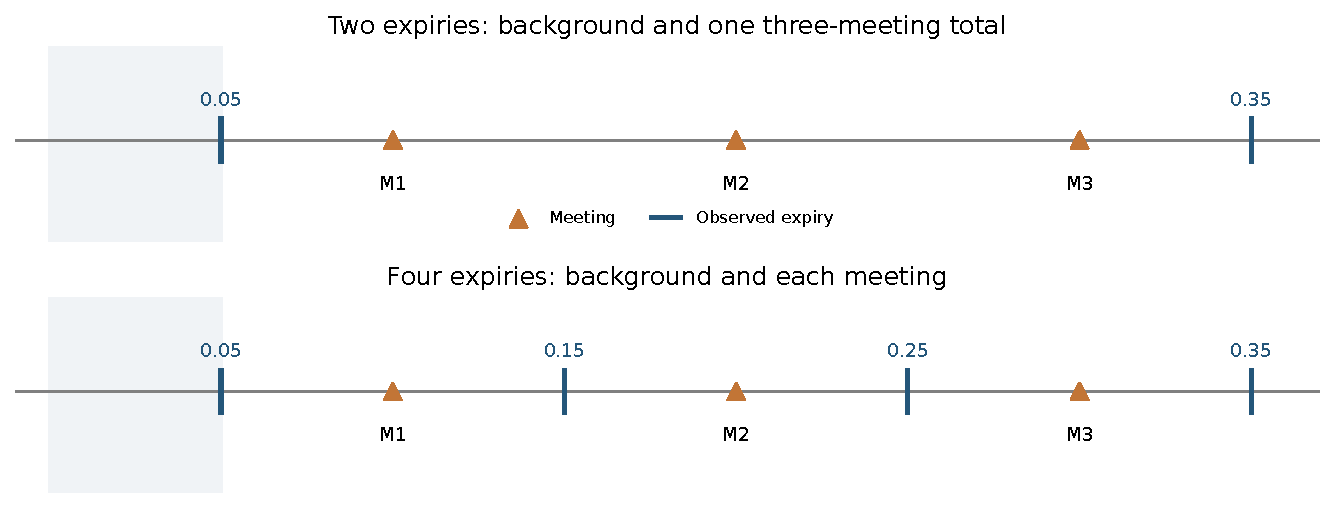
\includegraphics[width=.94\textwidth]{figures/calendar.pdf}
\caption{An expiry between meetings adds an independent variance observation. With constant background variance, the first meeting-free interval identifies the background. The sparse calendar identifies only the sum of the three meeting variances; the denser calendar separates them. Time is measured in years.}\label{fig:calendar}
\end{figure}

\subsection{Known maturity-dependent background loadings}\label{sec:shape}
A parallel diffusion is convenient but is not necessary for the calendar argument. Suppose its loading at time $s$ on forward maturity $T$ is $\sigma(s)\phi(s,T)$, where $\phi$ is known, bounded, and jointly Borel measurable on the finite horizon. Replace the continuous part of \eqref{eq:curve} by
\begin{equation}\label{eq:shapecurve}
\int_0^t\sigma(s)\phi(s,T)\,\dd W_s
+\int_0^t\sigma(s)^2\phi(s,T)\left(\int_s^T\phi(s,x)\,\dd x\right)\dd s.
\end{equation}
The deterministic drift is again the HJM drift. The meeting part remains the parallel-jump specification already defined.

For contract $\ell$, define its average diffusion loading
\[
\beta_\ell(s)=\frac1{\delta_\ell}\int_{a_\ell}^{b_\ell}\phi(s,x)\,\dd x,
\qquad 0\leq s\leq S_\ell.
\]
Its normalized log variance becomes
\begin{equation}\label{eq:shapeD}
\cV_\ell=\sum_{T_i\leq S_\ell}v_i+\sum_j\mathsf D_{\ell j}u_j,\qquad
\mathsf D_{\ell j}=\int_{[c_{j-1},c_j)\cap(0,S_\ell]}\beta_\ell(s)^2\,\dd s.
\end{equation}
Set $\mathsf D_{0j}=0$ and $\Delta \mathsf D_{\ell j}=\mathsf D_{\ell j}-\mathsf D_{\ell-1,j}$.

\begin{corollary}[Calendar criterion with a known shape]\label{cor:shape}
For \eqref{eq:shapeD}, Theorem~\ref{thm:rank} holds with $\Lambda_E$ replaced by $(\Delta \mathsf D_{\ell j})_{\ell\in E,j}$. In particular, for the strictly increasing expiry sequence considered here, at least $n_b$ meeting-free gaps remain necessary.
\end{corollary}
When adjacent options refer to different accrual windows, the differenced background row is not just the variance accumulated between their expiries. Earlier Brownian shocks can have different weights in the two contracts. Some coefficients in $\Delta\mathsf D$ can therefore be negative. For example, with $\phi(s,T)=e^{-\kappa(T-s)}$, $\kappa>0$,
\[
\beta_\ell(s)=\frac{1-e^{-\kappa\delta_\ell}}{\kappa\delta_\ell}
                  e^{-\kappa(a_\ell-s)}.
\]
Moving the underlying window farther out reduces the weight of an earlier shock. One must build $\mathsf D$ from the actual underlying windows before differencing. The corollary treats a known $\phi$; estimating its shape parameters creates an additional inverse problem. With several windows at the same expiry, build a row for each contract directly in \eqref{eq:shapeD}. Such rows have identical meeting entries but can have different background entries. They can therefore add background information under a nonparallel known shape, even though they add no new meeting cutoff.

\subsection{What futures quotes add}\label{sec:extra}
Theorem~\ref{thm:rank} deliberately uses only $\cV$. Proposition~\ref{prop:pricing} shows why a statement about all option and futures prices would be different. For the parallel diffusion and pre-accrual expiry,
\begin{equation}\label{eq:zrows}
\frac{z_\ell}{\delta_\ell}
=\sum_i(S_\ell-T_i)^+v_i+
  \sum_ju_j\int_{[c_{j-1},c_j)\cap(0,S_\ell]}(S_\ell-s)\,\dd s.
\end{equation}
The mean fitted from the cash option surface, together with its underlying futures quote, supplies this additional row. Known initial bond prices can supply the $p$ rows of \eqref{eq:p}. Full rank of the stacked observation matrix is the appropriate exact identification test for those richer data.

\begin{table}[ht]
\centering\small
\begin{tabular}{p{.34\textwidth}p{.56\textwidth}}
\toprule
Observations used & Model quantities available in the exact experiment\\
\midrule
Option-variance panel & $q_\ell$, hence $\cV_\ell$; calendar criterion applies directly.\\
Complete cash option surfaces & $P(0,S_\ell)$, $m_\ell$, and $q_\ell$.\\
Surfaces plus underlying futures & Additionally $z_\ell=\log G_{0,\ell}-\log m_\ell$.\\
Surfaces, futures, initial bond curve & Additionally $p_\ell=\log G_{0,\ell}-\int_{a_\ell}^{b_\ell}f_0$.\\
\bottomrule
\end{tabular}
\caption{Different observation sets require different identification claims. With a known initial curve, the two strikes in Proposition~\ref{prop:finitequotes} can replace each complete surface in this exact experiment. Finite price precision still requires bounds.}\label{tab:observations}
\end{table}

The extra information may be tiny in rate-price units. Move $100$ bp$^2$ of variance between two meetings separated by $1/12$ year while preserving the total. At a later expiry, \eqref{eq:zrows} changes $z$ by $\delta\times10^{-6}/12$. For a quarterly window this is about $2.1\times10^{-8}$. Holding $G_0$ fixed, the corresponding shift in the mean rate is about $G_0\times0.00083$ bp. With a known initial curve, the futures mean can also move, but on the same small scale for this perturbation. Exact nonzero information is not necessarily informative at a quarter-basis-point price tolerance. This arithmetic illustrates conditioning, not a general bound for every parameter direction.

Futures alone can identify in a deliberately designed pure-jump experiment. Suppose background volatility is zero and use windows $a_n=T_n<b_n<T_{n+1}$ (with $b_N>T_N$). Subtract the known initial-curve integral from $\log G_{0,n}$ to obtain $p_n$. Then
\[
v_n=\frac{p_n-\delta_n\sum_{i<n}(b_n-T_i)v_i}{\delta_n^2},\qquad
\delta_n=b_n-T_n.
\]
The coefficients are triangular because a later meeting occurs after the window ends. This identifies all meeting variances recursively. Standard quarterly futures do not supply these freely chosen windows. The result distinguishes insufficient instruments from an intrinsic inability of futures prices to contain variance information.

Appendix~\ref{app:listedcalendar} applies the rank criterion to actual versus hypothetical listing calendars. It also exhibits a known exponential loading for which an otherwise identifying background partition becomes singular at one positive decay rate, and a case where futures-mean observations restore exact rank while adding information far below the price tolerance. These examples are useful checks before interpreting a numerically unique calibration.

\section{When later contracts cannot recover earlier meeting allocations}\label{sec:aggregation}
The calendar result identifies a limitation of the variance panel. We now give a stronger result for a particular contract family, allowing many strikes, later cash flows, and American cash exercise. In this section set $f_0=0$ and $\sigma=0$ in \eqref{eq:curve}. Use the usual augmentation of the filtration generated by the meeting surprises alone. These restrictions isolate the information lost when observation and exercise begin only after a group of meetings. This is a separate exact experiment, not the model used for the empirical calibration.

Fix a future cutoff $A\geq T_k$, with exactly $k$ meetings at or before $A$. These meetings are still future events from time zero. Write
\begin{equation}\label{eq:VH}
V=\sum_{i\leq k}v_i,\qquad M_1=\sum_{i\leq k}T_i v_i,\qquad y=r_A.
\end{equation}
Hold later meeting dates and variances fixed. For $t\geq A$ and $T\geq t$, direct substitution gives
\begin{equation}\label{eq:postcurve}
f(t,T)=y+V(T-A)+\sum_{A<T_i\leq t}\{X_i+v_i(T-T_i)\}.
\end{equation}
The curve after $A$ therefore remembers the earlier surprises through the single random level $y$ and the deterministic total $V$. It does not retain their individual variances.

\begin{theorem}[Aggregation after a cutoff]\label{thm:aggregate}
In this pure-jump model the following statements hold.
\begin{enumerate}
\item Under the probability measure with density $B_A^{-1}$ relative to $\Q$, $y$ has law $N(0,V)$ and is independent of all later surprises. The density has expectation one.
\item Consider a cash flow paid at $S\geq A$ that is a fixed Borel function of the curve history from $A$ to $S$, using the same function when the earlier variance allocation changes. If its discounted absolute value is integrable, its time-zero value depends on the earlier variances only through $V$.
\item Let $Y_t$, $A\leq t\leq S$, be an American cash payoff given by a fixed Borel, nonanticipating rule of the post-$A$ curve history, with the same rule across allocations. Suppose the payoff discounted back to $A$, $\widehat Y_t=(B_A/B_t)Y_t$, is adapted, has right-continuous paths with left limits, and satisfies $\sup_{A\leq t\leq S}|\widehat Y_t|\leq\mathcal M$ for an integrable $\mathcal M$ under the tilted measure. Then $\sup_\tau\E[B_\tau^{-1}Y_\tau]$, over full-history stopping times $\tau\in[A,S]$, depends on the earlier variances only through $V$.
\item For continuously compounded futures on windows $[a,b]$ with $a\geq A$,
\begin{equation}\label{eq:futureVH}
\log G_0(a,b)=\delta(bV-M_1)+\text{known later-meeting contribution}.
\end{equation}
Consequently allocations with the same $(V,M_1)$ give all the same values in this stated family. If the observations include two such futures with distinct terminal dates $b$, they determine $(V,M_1)$.
\end{enumerate}
\end{theorem}
The qualification that the payoff rule is the same is substantive. A claim that explicitly pays the unobserved parameter $v_1$, or a rule whose strike changes with $M_1$, is not a fixed contract in this family. The total $V$ may enter the payoff through the observed curve, including its slope; an allocation-dependent payoff rule is excluded. Ordinary fixed-strike cash claims on that curve satisfy the requirement.

The proof of the American statement does not assert that exercise is European or that early exercise has no value. It shows that the extra information about individual early surprises is independent randomization after the change of measure, and cannot improve the supremum over stopping rules. The path regularity and domination in part 3 permit approximation of continuous exercise by finite exercise grids; standard continuous-payoff cash options satisfy these sufficient conditions in this finite Gaussian model. Appendix~\ref{app:aggregation} gives the argument. Actual exchange delivery into futures positions is a separate contract convention.

The European result also covers products of bond-implied overnight accumulation factors after $A$. Define a fixing on $[u_j,u_{j+1}]$ by $L_j=(P(u_j,u_{j+1})^{-1}-1)/(u_{j+1}-u_j)$. Its product $\prod_j(1+(u_{j+1}-u_j)L_j)$ is a function of the post-$A$ curve. It equals $\exp(\int_a^b r_s\,\dd s)$ in this pure-jump model if no meeting lies strictly inside any fixing interval. Without that alignment the aggregation statement for the payoff still holds, but formula~\eqref{eq:futureVH} is not being asserted for the product. Bond-implied fixings are a model convention, not an identification with every realized SOFR fixing.

\subsection{The set of compatible allocations}
Given $(V,M_1)$, the possible early-meeting vectors are exactly
\begin{equation}\label{eq:polytope}
\Pi(V,M_1)=\left\{x\in\R_+^k:\ \sum_i x_i=V,\quad \sum_i T_i x_i=M_1\right\}.
\end{equation}
For $V\geq0$, this set is nonempty if and only if $T_1V\leq M_1\leq T_kV$. If $V=M_1=0$, it consists only of the zero vector. If $V>0$, it is compact. If it contains a strictly positive vector and $k\geq2$, its dimension is $k-2$: the two equality rows are independent because the meeting dates are distinct, and nonnegativity imposes no local restriction at that vector. Every coordinate reaches its minimum and maximum at an allocation with at most two positive coordinates. For a pair $i<j$, the candidate allocation is
\begin{equation}\label{eq:vertices}
x_i=\frac{T_jV-M_1}{T_j-T_i},\qquad
x_j=\frac{M_1-T_iV}{T_j-T_i},
\end{equation}
when both are nonnegative, with all other coordinates zero. A one-coordinate allocation is possible when $M_1=T_iV$. These candidates give sharp bounds by a finite calculation.

For three equally spaced meetings at $T_i=i/12$, $V=700$ bp$^2$, and $M_1=2V/12$, the set is
\[
(x_1,x_2,x_3)=(x,700-2x,x),\qquad 0\leq x\leq350.
\]
The two allocations in the introduction lie on this same line. The second meeting can have any variance between zero and $700$ bp$^2$, while preserving all observations in Theorem~\ref{thm:aggregate}. The bounds on different meetings are joint constraints: their coordinate intervals cannot be combined arbitrarily.

\begin{figure}[ht]
\centering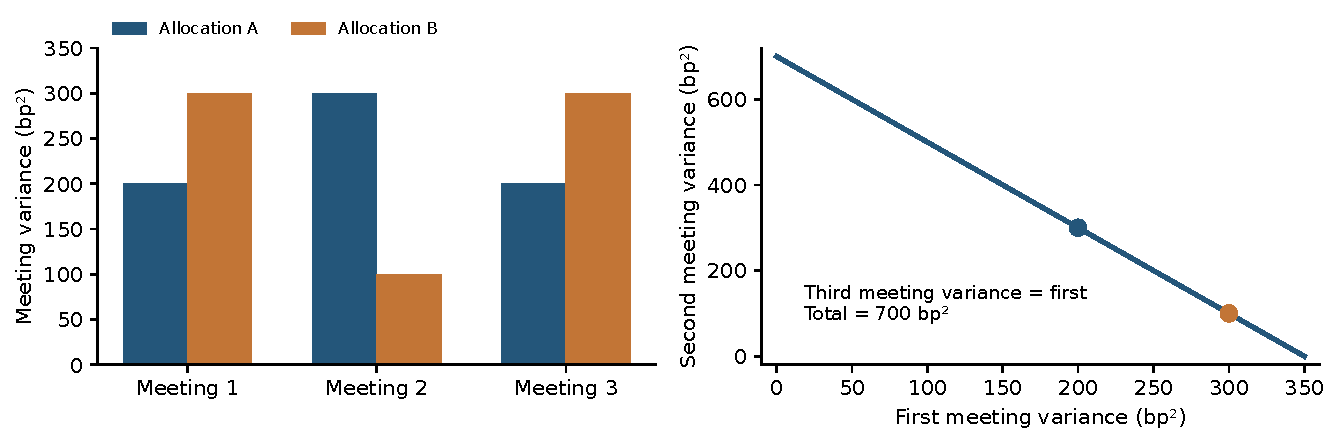
\includegraphics[width=.95\textwidth]{figures/aggregation.pdf}
\caption{Two different allocations with the same prices for the contract family in Theorem~\ref{thm:aggregate}. Left: the two allocations. Right: the entire compatible set for the first two coordinates; the third equals the first. The meeting dates are equally spaced.}\label{fig:aggregate}
\end{figure}

\subsection{A deterministic initial curve and continuous pre-cutoff risk}
The aggregation mechanism is not tied to a zero initial curve or to an absence of background volatility. The following extension connects it to the model of Section~\ref{sec:prices}. Keep the initial curve and all post-$A$ parameters fixed, and allow both the earlier meeting variances and the deterministic background volatility before $A$ to vary. Define
\begin{equation}\label{eq:generalaggregates}
V_A=\sum_{T_i\leq A}v_i+\int_0^A\sigma(s)^2\,\dd s,\qquad
M_{1,A}=\sum_{T_i\leq A}T_i v_i+\int_0^A s\sigma(s)^2\,\dd s.
\end{equation}
For this extension use the usual augmentation (completion and right-continuous regularization) of the natural filtration generated by
$Y_t=\int_0^t\sigma(s)\,\dd W_s$ and the meeting surprises revealed by time $t$. Thus exercise uses the history of the model's driving risks. The statement below does not allow an arbitrary larger filtration.

\begin{corollary}[Aggregation including continuous risk]\label{cor:generalaggregate}
For the model \eqref{eq:curve}, under the probability measure with density
$B_A^{-1}/P(0,A)$, the centred level $y_A=r_A-f_0(A)$ is $N(0,V_A)$ and independent of future driving increments. Fixed post-$A$ cash claims depend on the pre-$A$ variance allocation only through $V_A$, including American claims under the regularity and domination assumptions of Theorem~\ref{thm:aggregate}. For $a\geq A$,
\[
\log G_0(a,b)=\int_a^b f_0(x)\,\dd x+\delta(bV_A-M_{1,A})
                   +\text{fixed post-$A$ contribution}.
\]
Thus equal $(V_A,M_{1,A})$ gives equal prices for the same post-cutoff contract family.
\end{corollary}
\begin{proof}
Write $L_A=\int_0^A\sigma\,\dd W+\sum_{T_i\leq A}X_i$. Then
$y_A=L_A+AV_A-M_{1,A}$, and the normalized discount density is the Gaussian exponential with random exponent
\[
-\int_0^A(A-s)\sigma(s)\,\dd W_s-\sum_{T_i\leq A}(A-T_i)X_i.
\]
Its covariance with $L_A$ is $-(AV_A-M_{1,A})$. Exponential tilting therefore centres $y_A$ and preserves its variance $V_A$. For $t\geq A$,
\begin{align*}
f(t,T)={}&f_0(T)+y_A+V_A(T-A)+\int_A^t\sigma(s)\,\dd W_s\\
&+\int_A^t\sigma(s)^2(T-s)\,\dd s
  +\sum_{A<T_i\leq t}\{X_i+v_i(T-T_i)\}.
\end{align*}
For a nonnegative Borel cash payoff, integration against this state law gives a value depending on the earlier allocation only through $V_A$, multiplied by the fixed factor $P(0,A)$. An absolutely integrable signed payoff is the difference of its positive and negative parts, so the same conclusion follows by applying the nonnegative result twice.

For American exercise, when $V_A>0$, regress the early Gaussian history onto $y_A$ under the tilted measure. The centred residual history is independent of $y_A$ and of all future driving increments. Continuity of $Y$ allows its history to be recovered from rational-time coordinates, together with the finitely many revealed surprises. At each time $s\geq A$, the completed natural information therefore equals that generated by the residual history, $y_A$, and the driving increments from $A$ to $s$, with the same null sets adjoined. The strictly positive discount density preserves those null sets. Take right-continuous regularizations on both sides to obtain the exercise filtration.

Section a finite-grid stopping rule at each fixed residual history. Independence bounds its expectation by the supremum over rules using only $y_A$ and the future driving increments; those rules also give the reverse inequality. Upward grid approximation, right-continuity, and dominated convergence under the assumed integrable envelope extend the equality to continuous exercise. The envelope can be taken as the supremum of the discounted payoff over rational times and the terminal time, a Borel function of the post-cutoff state history. Consequently the value depends only on that history's law and $V_A$. When $V_A=0$, $y_A$ is deterministic and the same sectioning argument applies to the independent residual history. Finally $h(s)=\delta(b-s)$ before $A\leq a$ in \eqref{eq:p}, proving the futures identity.
\end{proof}
When pre-cutoff background variance is fixed, subtract its known total and first moment to recover the meeting-allocation polytope \eqref{eq:polytope}. When it is also unknown, the indistinguishable set includes both meeting allocations and continuous variance profiles with the same two moments. Later cash contracts cannot separate those components.

\subsection{Exercise convention changes value, but need not restore identification}
The pure-jump model gives an explicit cash-exercise formula after the last meeting. Let $T_N\leq A<S\leq a<b$, $\bar t=(a+b)/2$, and $L=S-A$. The futures rate is already known at $A$ and remains constant thereafter:
\[
F_t=\frac{\exp\{\delta r_A+\delta V(\bar t-A)\}-1}{\delta},
\qquad A\leq t\leq b.
\]
For $V>0$, define
\[
\mathcal D_{V,L}(x)=\max_{0\leq u\leq L}e^{-xu-Vu^2/2},\qquad
u_*(x)=\min\{L,\max\{0,-x/V\}\}.
\]
A call with rate strike $k$ and cash paid on exercise has value
\begin{equation}\label{eq:latecash}
U=\E_{Y\sim N(0,V)}
 \left[\left(\frac{e^{\delta Y+\delta V(\bar t-A)}-1}{\delta}-k\right)^+
                         \mathcal D_{V,L}(Y)\right].
\end{equation}
Indeed, $B_{A+u}/B_A=e^{r_Au+Vu^2/2}$; the known nonnegative payoff is maximized after discounting by exercise at $A+u_*(r_A)$. Tilting to $A$ gives \eqref{eq:latecash}. For every finite strike and $V>0$, cash exercise strictly improves on mandatory exercise at $S$: on a sufficiently large positive-$r_A$ set the call pays and immediate exercise discounts less. Yet its value still contains no information about individual earlier variances beyond $V$.

For comparison, define the futures-style exercise functional
\[
\widetilde U=\sup_{\tau\in\mathcal T[A,S]}\E[(F_\tau-k)^+],
\]
without cash discounting. Since $F$ is a martingale and the payoff is convex, conditional Jensen and optional sampling give
\begin{equation}\label{eq:futuresstyle}
\widetilde U=\E[(F_S-k)^+]
 =\frac1\delta\mathcal B\left(G_0,1+\delta k,
                         \sum_{T_i\leq S}w(T_i)^2v_i\right)
\end{equation}
for $1+\delta k>0$, with the intrinsic linear formula otherwise. This holds even when exercise spans unrevealed meetings; Gaussian exponential moments supply the required integrability. The no-early-exercise conclusion is the established result of \citet{lieu1990option,chen1993pricing}. Its identification consequence here is that earlier variances still enter only through $(V,M_1)$ when accrual starts after the cutoff. Additional expiries can identify later meetings with nonzero $w(T_i)$, but cannot resolve the earlier polytope.

The two formulas distinguish cash timing value from information about the earlier allocation. They do not identify the undiscounted functional with CME's premium-paid option convention. Exact cash exercise across one unrevealed meeting is given in Appendix~\ref{app:crossmeeting}; it depends on the earlier total and the crossed meeting variance separately.

\section{Price precision and sharp risk ranges}\label{sec:precision}
\subsection{Invert prices before differencing variances}
Even an identifying calendar can produce unstable estimates. A meeting variance is obtained by subtracting accumulated variances at two expiries and subtracting estimated background variance. Each term can be much larger than their difference.

For a pre-accrual expiry $S<a$, there is a simple exact inversion for a cash option struck at its forward-measure mean $K=m$. Keep its discount factor $D=P(0,S)>0$, mean $m$, and window length $\delta$ fixed. The premium per unit rate, $c=C/\delta$, satisfies
\begin{equation}\label{eq:atm}
c=\frac{Dm}{\delta}\left[2\Phi\left(\frac{\delta\sqrt{\cV}}{2}\right)-1\right].
\end{equation}
This is strictly increasing in $\cV\geq0$. Its inverse is
\begin{equation}\label{eq:inverse}
\mathcal I(c;D,m,\delta)=\frac4{\delta^2}
 \left[\Phi^{-1}\left(\frac{1+\delta c/(Dm)}2\right)\right]^2,
 \quad 0\leq c<Dm/\delta.
\end{equation}
An admissible premium interval $[\underline c,\overline c]$ gives an exact variance interval $[\mathcal I(\underline c),\mathcal I(\overline c)]$. Clip a negative lower premium bound at zero. An upper premium bound at or above $Dm/\delta$ gives no finite upper bound on $\cV$, provided the interval contains an attainable premium. If its lower bound is at or above that ceiling, or its upper bound is negative, the interval is incompatible with every finite $\cV$.

These are conditional bounds for the variance observation: $D$, $m$, and the strike $K=m$ are fixed inputs. A quoted strike near $m$ is not exactly at the money in this sense. For a fixed non-ATM strike one instead numerically inverts the monotone Black formula. When $D$ and $m$ are estimated, their uncertainty must be carried through the inversion or retained in a joint price-feasibility problem. The closed-form formula is not a justification for ignoring it.

\subsection{A feasible set, rather than a single allocation}
Suppose inversion or surface fitting supplies bounds $\underline{\cV}_\ell\leq \cV_\ell\leq\overline{\cV}_\ell$. Define
\begin{equation}\label{eq:feasible}
\Theta=\{\theta\geq0:\ \underline{\boldsymbol{\cV}}\leq\mathsf A\theta
                                    \leq\overline{\boldsymbol{\cV}}\}.
\end{equation}
For any requested linear quantity $c^\top\theta$, calculate
\begin{equation}\label{eq:LP}
\underline r(c)=\inf_{\theta\in\Theta}c^\top\theta,\qquad
\overline r(c)=\sup_{\theta\in\Theta}c^\top\theta.
\end{equation}
These are linear programs. They give sharp bounds for the stated observation intervals and model: every feasible value respects all inequalities, and no narrower bounds can contain the feasible set. Infinite endpoints signal a genuinely unbounded exposure. If $\Theta$ is nonempty and bounded, both endpoints are attained. Additional linear observations, including bounds on $z$ and $p$, can be stacked with the variance rows. Box bounds obtained separately from correlated observations remain valid outer bounds, but may then be conservative relative to their joint price information. In particular, fixing $m$ in the inversion does not enforce its structural identity $m=G_0e^{-z(\theta)}$. If $G_0$ and $m$ are both treated as observed, their implied $z$ restriction must also be imposed. Without it, \eqref{eq:LP} is sharp for the retained variance intervals, not necessarily for all observed cash and futures prices.

A point estimate can still be useful. For example, nonnegative weighted least squares minimizes
\begin{equation}\label{eq:fit}
\sum_{\ell=1}^L w_\ell((\mathsf A\theta)_\ell-\widehat{\cV}_\ell)^2,
\qquad \theta\geq0,\quad w_\ell>0.
\end{equation}
It selects a representative fit. It does not turn a non-identifying panel into an identifying one. A smoothness penalty or a prior supplies additional information from the modeller. Report its effect by comparing the feasible ranges before and after imposing it.

An empty feasible set also has an interpretation: the chosen observations, tolerances, and model are incompatible. It does not identify which input is wrong. Check units, underlying-contract mappings, exercise conventions, and distributional fit before enlarging tolerances. Silently forcing negative meeting variances to zero can hide this diagnosis.

\subsection{Exact bounds in a cumulative special case}
When background variance is zero and exactly one new meeting occurs between consecutive observed expiries, the problem admits closed forms. Let $\cV_n=\sum_{i\leq n}v_i$, with $\cV_0=0$, and suppose finite intervals $\ell_n\leq \cV_n\leq r_n$ are given, where $0\leq\ell_n\leq r_n$. Define
\begin{equation}\label{eq:envelopes}
L_n=\max_{i\leq n}\ell_i,\qquad R_n=\min_{j\geq n}r_j,
\qquad L_0=R_0=0.
\end{equation}
\begin{proposition}[Sharp cumulative bounds]\label{prop:cumulative}
There exists a feasible nonnegative meeting-variance vector if and only if $L_n\leq R_n$ for every $n$. When feasible, the sharp interval for $v_n$ is
\begin{equation}\label{eq:cumbounds}
\max\{0,L_n-R_{n-1}\}\ \leq v_n\leq R_n-L_{n-1}.
\end{equation}
\end{proposition}
Thus the information from later prices can tighten an earlier cumulative upper bound, and earlier prices can tighten a later cumulative lower bound. Inverting each price and independently differencing its endpoints without enforcing monotonicity can miss this tightening. The linear programs in \eqref{eq:LP} handle the general case with background variance and multiple meetings per gap.

\subsection{A quick local precision calculation}
Differentiating \eqref{eq:atm} gives the first-order response of $\cV>0$ to a premium error of size $\varepsilon$ in decimal rate units:
\begin{equation}\label{eq:eta}
\eta(\cV)=\frac{2\varepsilon\sqrt{\cV}}
 {Dm\,\varphi(\delta\sqrt{\cV}/2)}.
\end{equation}
This is a local approximation; use \eqref{eq:inverse} for finite intervals. When $\delta\sqrt{\cV}$ is small, the denominator's normal density is close to $1/\sqrt{2\pi}$. Uncertainty in variance then grows roughly in proportion to the total accumulated standard deviation, even if the variance of the particular meeting of interest remains small.

For one constant background variance rate, suppose the first gap is meeting-free and meeting $i$ is alone in gap $\ell\geq2$. With gap length $g_\ell=S_\ell-S_{\ell-1}$, the exact estimator is
\[
\widehat u=\widehat{\cV}_1/g_1,\qquad
\widehat v_i=\widehat{\cV}_\ell-\widehat{\cV}_{\ell-1}-g_\ell\widehat u.
\]
If the variance errors range over the Cartesian box $|\Delta \cV_j|\leq\eta_j$, its sharp unrestricted linear error bound is
\begin{equation}\label{eq:differror}
|\Delta\widehat v_i|\leq\eta_\ell+\eta_{\ell-1}
                                      +(g_\ell/g_1)\eta_1.
\end{equation}
For $\ell=2$, the two occurrences of the first observation combine with the same sign. Nonnegativity and additional observations can tighten this linear bound. A short first meeting-free gap creates a noisy estimate of $u$, and that error is multiplied by the length of each subsequent gap.

More generally, a linear estimator $a^\top\widehat{\boldsymbol{\cV}}$ recovers $c^\top\theta$ exactly in the noiseless model if $\mathsf A^\top a=c$. Its worst-case box-error bound is $\sum_\ell|a_\ell|\eta_\ell$. Minimizing this expression subject to $\mathsf A^\top a=c$ is another linear program after splitting positive and negative parts. It compares linear estimators for an already identified quantity; it neither replaces the nonlinear price inversion nor supplies information about a quantity outside the row space.

\section{Restrictions that survive factor calibration}\label{sec:restrictions}
An option panel restricts meeting risk through its observation map. A factor specification imposes a second restriction: some variance vectors cannot occur at any calibration. We determine that set for deterministic scales, and the exact support of the random variance vector for square-root stochastic scales. These results concern the scheduled short-rate model of \citet{brace2024sofr}, rather than an extra assumption on the independent announcement model of Section~\ref{sec:prices}.

The distinction between the constructions matters. In Section~\ref{sec:prices}, the forward curve itself jumps at a meeting. Below, each fixed-maturity forward rate is continuous in time; the short rate jumps when its maturity passes a scheduled discontinuity in the forward curve. The conditional variance of that short-rate jump is the quantity compared across models.

A scalar announcement state can coexist with arbitrarily many free meeting-variance parameters; restrictions arise from the specified loadings and scales, not from state dimension alone.

\subsection{All restrictions under deterministic scale recalibration}
Write $\nu(s)=\#\{i:T_i\leq s\}$, and set $T_0=0$. Factor $j$ has fixed ordinal loadings $\gamma_{i,j}$, constant decay $\kappa_j\geq0$, and deterministic scale $a_j(s)$. Its loading on the short-rate jump at meeting $n$ is
\[
g_{nj}(s)=a_j(s)e^{-\kappa_j(T_n-s)}\gamma_{n-\nu(s),j},\qquad s<T_n.
\]
Independent Brownian factors and the deterministic HJM drift give
\begin{equation}\label{eq:detvariance}
\boldsymbol V_n(t):=\Var_Q(\Delta r_{T_n}\mid\F_t)
 =\sum_j\int_t^{T_n}g_{nj}(s)^2\,\dd s,\qquad t<T_n.
\end{equation}
Bold $\boldsymbol V(t)$ denotes the vector across future meetings; the scalar $V$ in Section~\ref{sec:aggregation} remains a sum of announcement variances.

Fix $t$, all dates, loadings, and decays. Partition the remaining horizon into meeting intervals $I_k=[\max(t,T_k),T_{k+1})$, $k=\nu(t),\ldots,N-1$. Define the nonnegative matrix
\begin{equation}\label{eq:scale-matrix}
\mathsf K_{n,(j,k)}(t)=\ind_{\{n>k\}}\gamma_{n-k,j}^2
 \int_{I_k}e^{-2\kappa_j(T_n-s)}\,\dd s.
\end{equation}
Rows correspond to future meetings; columns correspond to factor--interval pairs.

\begin{theorem}[Restrictions surviving all scale choices]\label{thm:scales}
Allow each $a_j$ to be any nonnegative Borel function bounded on finite horizons. The set of attainable vectors in \eqref{eq:detvariance} is exactly
\begin{equation}\label{eq:cone}
\mathcal K(t)=\{\mathsf K(t)\eta:\eta\geq0\}.
\end{equation}
Consequently $\omega^\top\boldsymbol V(t)\geq0$ holds under every scale calibration if and only if $\omega^\top\mathsf K(t)\geq0$ componentwise. These inequalities characterize attainability. For one factor with $\gamma_{1,1}\ne0$, $\mathsf K$ is square and lower triangular with positive diagonal, and membership is equivalent to $\mathsf K^{-1}\boldsymbol V\geq0$.

If each factor has constant ordinal loadings, $\gamma_{i,j}=\gamma_j\ne0$, put $\kappa_{\max}=\max_j\kappa_j$. The complete restrictions then reduce to
\begin{equation}\label{eq:surviving-ratios}
\boldsymbol V_{\nu(t)+1}(t)\geq0,\qquad
\boldsymbol V_n(t)\geq e^{-2\kappa_{\max}(T_n-T_{n-1})}
                         \boldsymbol V_{n-1}(t).
\end{equation}
Every vector satisfying these inequalities is attainable using only a factor with decay $\kappa_{\max}$.
\end{theorem}
\begin{proof}
On $I_k$, the vector integrand in \eqref{eq:detvariance} is $a_j(s)^2e^{2\kappa_js}$ times the fixed vector with entries $\ind_{\{n>k\}}e^{-2\kappa_jT_n}\gamma_{n-k,j}^2$. Its integral is a nonnegative multiple of the corresponding column of $\mathsf K$. Every multiple is attained by a constant squared scale on $I_k$. This proves equality with the finitely generated closed cone. Separation gives the dual inequalities. The one-factor diagonal entries are strictly positive.

For constant ordinal loadings, the contribution of factor $j$ satisfies
\[
\boldsymbol V_n^{(j)}=e^{-2\kappa_j(T_n-T_{n-1})}\boldsymbol V_{n-1}^{(j)}
                         +\mathsf K_{n,(j,n-1)}\eta_{j,n-1}.
\]
Summing proves necessity of \eqref{eq:surviving-ratios}. For sufficiency, use a fastest-decaying factor and choose its successive squared scales to equal the nonnegative residual in this equation divided by the positive diagonal entry.
\end{proof}

Refining the scale partition adds no new vectors once it contains all meeting dates. Time-varying scales can remove the equality restrictions of a constant-scale model while leaving exact inequalities. At zero decay and constant ordinal loading, no scale choice can make meeting variance decrease with the meeting index. With consecutive meetings $1/8$ year apart and all decays bounded by $1$ per year, a fall from $400$ to $200$ bp$^2$ is impossible: the second variance must be at least $400e^{-1/4}=311.5$ bp$^2$.

The bound survives joint recalibration of scales and decays in $[0,\bar\kappa]$: replace $\kappa_{\max}$ by $\bar\kappa$ in \eqref{eq:surviving-ratios}, and a factor with decay $\bar\kappa$ attains every allowed vector. Unbounded decays make the closure of the attainable union the nonnegative orthant. Freely varying ordinal loadings gives the entire orthant already at fixed decay, by choosing only $\gamma_{1,1}$ nonzero so that $\mathsf K$ is diagonal. The ratio formula is for constant ordinal loadings; for the general loadings in \citet{brace2024sofr}, use \eqref{eq:scale-matrix} and its dual inequalities.

\subsection{Exact restrictions under stochastic volatility}
Replace deterministic factor variance by a square-root state $Z_j$, starting from one:
\begin{equation}\label{eq:svstate}
\dd Z_j(s)=\vartheta_j(1-Z_j(s))\,\dd s
                +\alpha_j(s)\sqrt{Z_j(s)}\,\dd U_j(s),\qquad Z_j(0)=1.
\end{equation}
Here $\vartheta_j\geq0$ is constant and $\alpha_j\geq0$ is piecewise constant with finitely many pieces on bounded intervals. The Brownian pairs $(W_j,U_j)$ are independent across factors, with $\dd[W_j,U_j]_s=\rho_j(s)\,\dd s$, $|\rho_j(s)|\leq1$. Assume adapted nonnegative continuous solutions, $\E\sup_{s\leq H}Z_j(s)^2<\infty$, and predictable square-integrable noise and forward-loading integrands on each finite horizon. Existence of these solutions is a hypothesis.

The conditional meeting-variance vector has the affine form
\begin{equation}\label{eq:svmap}
\boldsymbol V(t)=\boldsymbol c(t)+\mathsf L(t)Z(t),
\end{equation}
with deterministic nonnegative coefficients
\[
\mathsf L_{nj}(t)=\int_t^{T_n}\mathcal H_{nj}(u)e^{-\vartheta_j(u-t)}\,\dd u,
\qquad
\boldsymbol c_n(t)=\sum_j\int_t^{T_n}\mathcal H_{nj}(u)(1-e^{-\vartheta_j(u-t)})\,\dd u.
\]
Here $\mathcal H_{nj}$ is the squared effective noise loading for meeting $n$ and factor $j$, including the random HJM drift and its covariance with the forward noise. Appendix~\ref{app:svderivation} gives its explicit expression and derives the map. The diffusion loading alone does not give the actual conditional jump variance when that drift is random.

A containing cone need not be the actual support of a random vector. The square-root transition laws determine which columns of $\mathsf L$ are active and prove equality with a translated cone.

\begin{theorem}[Exact stochastic-volatility support]\label{thm:svsupport}
Fix $t>0$ and retain the meetings after $t$. Let $J$ contain the factors for which $\alpha_j>0$ on an interval of positive length before $t$. For $j\in J$, let $\ell_j$ be zero if a stochastic piece ends at $t$; otherwise propagate zero through the final deterministic pieces using $x\mapsto1+(x-1)e^{-\vartheta_j h}$. Set $\ell_j=1$ for $j\notin J$. Then
\begin{align}
\operatorname{supp}\boldsymbol V(t)&=\boldsymbol c(t)+\mathsf L(t)\ell
                                      +\mathsf L_J(t)\R_+^J,\label{eq:support}\\
\operatorname{aff}\operatorname{supp}\boldsymbol V(t)&=\boldsymbol c(t)+\mathsf L(t)\ell
                                      +\operatorname{range}\mathsf L_J(t),\nonumber\\
\Cov_Q(\boldsymbol V(t))&=\sum_{j\in J}\Var_Q(Z_j(t))\mathsf L_{\cdot j}(t)
                                      \mathsf L_{\cdot j}(t)^\top.\nonumber
\end{align}
Every variance in this sum is positive. Thus the covariance rank and affine-hull dimension both equal $\rank\mathsf L_J(t)$, and all almost-sure affine equalities are exactly the left-nullspace equalities of $\mathsf L_J(t)$ about the displayed vertex.
\end{theorem}
The proof, including the conditional version and boundary atoms, is in Appendix~\ref{app:support}. Its square-root transition input is classical; see \citet{malham2008square}. The result here determines the support of the actual meeting-variance vector with the full kernel \eqref{eq:svkernel}, including deterministic terminal pieces and inactive factors.

Appendix~\ref{app:bgsmapping} gives an equation-by-equation mapping to \citet{brace2024sofr} and applies the theorem to both columns of its Table~2. The constant specification has at most two active support directions; the time-dependent specification has at most three. These are restrictions at fixed parameters. Daily recalibration changes the affine map.

A polyhedral set of candidate meeting variances can be intersected with the deterministic cone by writing its meeting block as $\mathsf K\eta$, $\eta\geq0$. Feasibility and linear risk bounds remain linear programs. This tests the imposed variance restriction together with the chosen observation equations. The scheduled-rate factor model has dependent meeting risks and continuous fixed-maturity forwards; it does not inherit the independent-announcement model's option-pricing map. Testing its restrictions directly against prices requires its own pricer. The empirical analysis below therefore uses the announcement-calendar observation matrices, not a purported empirical test of the factor-support theorem.

\section{A calibration workflow and reproducible examples}\label{sec:calibration}
\subsection{What to collect and what to report}
A single cross-section suffices for a calibration illustration. It does not suffice to establish stability through time, estimate a physical risk premium, or compare hedging performance. For the cross-section, collect settlement date, exact option expiry, option type, strike, settlement premium, underlying futures identifier and settlement, and the underlying accrual start and end dates. Retain volume or open interest as context, rather than interpreting their presence as proof that a settlement is an executable quote. Add the meeting schedule and, for discounted cash pricing, the discount curve.

The following workflow implements the distinction between fit and identification.
\begin{enumerate}
\item \emph{Map contracts before fitting.} Serial options and quarterly options can reference the same underlying future. The option month is not its accrual window. Convert all premiums to one rate unit and use a consistent day count. Listed futures options use a price index that falls as the implied rate rises; a call on that index corresponds to a put on the rate after changing the strike and scale.
\item \emph{Specify the pricing experiment.} State whether the pricer treats European cash exercise or the actual listed exercise convention. State the assumed background variance schedule and maturity loadings. List any parameters imported from historical estimation.
\item \emph{Extract a small set of price quantities.} Fit the surface parameters $(D,m,q)$, or bound them over acceptable price errors. Inspect variation of implied variance across strikes. Under the Gaussian specification, systematic smile residuals indicate misspecification.
\item \emph{Construct the observation matrix.} Use the actual observed expiries and windows, compute its rank, and identify its row space. Add futures-assisted rows only if their price uncertainty is also retained.
\item \emph{Fit and bound.} Report a nonnegative fit and the extrema of individual variances and relevant group totals over the feasible set. Repeat under specified price tolerances and a small number of economically distinct background assumptions.
\item \emph{Check omitted prices and disclose failure.} Compare with strikes or expiries excluded from calibration. If no parameter vector fits the enlarged set at the stated tolerance, report that fact separately from the ranges obtained using the calibration subset.
\end{enumerate}
Historical bid--ask data are not an input to these steps. If current executable quotes are available, their spreads can inform the price intervals. With settlements alone, use disclosed tolerance scenarios. An interval of one or two settlement increments is an assumption about acceptable price error, not an estimate of a historical spread, transaction cost, or confidence level.

\subsection{A controlled variance-panel precision example}\label{sec:synthetic}
Take five meetings spaced $0.10$ year apart, from $0.10$ through $0.50$. Observe six option expiries spaced $0.10$ year apart, from $0.05$ through $0.55$. All options refer to the accrual window $[1,1.25]$. Each meeting has variance $100$ bp$^2$, and the constant background variance rate is $2{,}500$ bp$^2$ per year. The initial forward curve is flat at $4\%$. The first gap contains no meeting and each later gap contains exactly one, so Theorem~\ref{thm:rank} gives exact identification of all six parameters.

Generate the European prices from Proposition~\ref{prop:pricing}. For this controlled precision experiment, keep each discount factor and forward-measure mean fixed at its model value and use a strike equal to that mean. This fixes the nonlinear price-to-variance conversion while isolating uncertainty in the variance panel. We deliberately do not impose the additional model equations linking those means to the candidate variances and futures prices. The exercise is therefore an exact calculation for the extracted variance intervals, rather than a joint recalibration of every generated price. The generated cumulative variances are $125,475,825,1175,1525,1875$ bp$^2$. Invert premium intervals exactly by \eqref{eq:inverse}, and solve \eqref{eq:LP} for each meeting variance and the background rate.

Figure~\ref{fig:precision} shows the resulting sharp variance-panel ranges at premium tolerances of $0.25$ and $0.5$ rate basis points. At $0.25$ bp, the first meeting range is $[30.3,168.1]$ bp$^2$, while the fifth is $[0,231.3]$ bp$^2$. At $0.5$ bp, all five individual ranges include zero. Although every meeting is isolated by an expiry, finite price precision leaves wide intervals around the true value of $100$ bp$^2$. Later intervals are affected by the larger total accumulated uncertainty. The uncertainty in the background, learned from a short first gap, also propagates into every meeting estimate.

\begin{figure}[ht]
\centering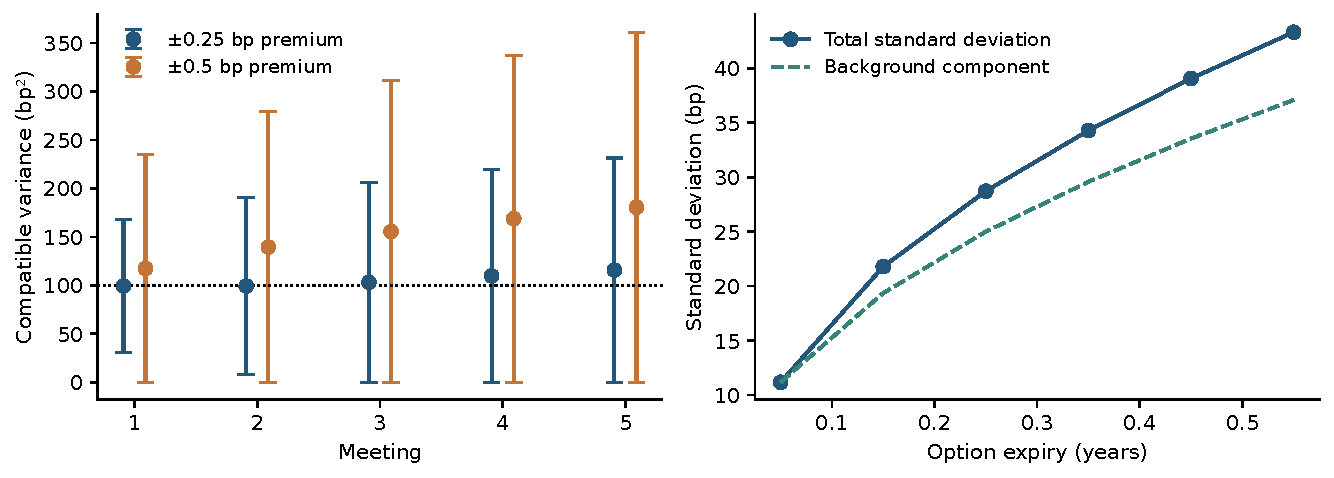
\includegraphics[width=.96\textwidth]{figures/precision.pdf}
\caption{Synthetic European variance-panel example. Left: sharp individual meeting-variance ranges for the extracted variance intervals, using fixed option means and discount factors for inversion; the dotted line is the true variance. Right: accumulated standard deviation and its background component. Full rank does not imply narrow ranges at finite price precision.}\label{fig:precision}
\end{figure}

All inputs and endpoint calculations are generated by the accompanying script. No simulation error enters this example. The price intervals are deterministic perturbation sets; they do not purport to contain a true parameter with a specified probability.


The next section applies the same sequence---contract mapping, fit checks, and feasible ranges---to a historical settlement panel. Section~\ref{sec:uses} then considers how those outputs can inform relative-value screening and hedge construction.

\section{Evidence from public SOFR settlements}\label{sec:market}\label{sec:empirical}
The empirical exercise asks whether an available option panel supports the meeting-risk allocations that a calibration would report. It separates three questions: which variances the contract calendar can distinguish, whether a specified pricing approximation fits, and which allocations remain possible when it does. The principal findings are that the full meeting vector is never identified by the selected variance panel, that fitting one strike can conceal sizeable errors at other strikes, and that a positive lower bound on a meeting variance can disappear when the background is made more flexible.

\subsection{Data and a fixed selection rule}
The starting panel contains 20,498 matched call--put strike pairs on 78 trading dates from 30 March through 14 September 2026. Each pair has numerical settlements for both sides and its underlying SR3 future from same-date \emph{final} CME Daily Bulletins. The archive is irregular: it is not a complete daily record. Matching uses the trading date printed inside each PDF, rather than the archive capture date. Cabinet quotes and blank settlements are retained in the source extraction but excluded from the matched panel. All 3,793 comparisons of extracted standard-option volume and open interest with printed contract totals agree. Missing archive captures, missing paired final sections, and the need for numerical settlements determine date availability before the calibration screen. Ten of the 78 retained dates lie within three calendar days of an FOMC decision, compared with 16 of the 121 weekdays in the sample span (before exchange-holiday exclusions). This simple comparison shows no obvious concentration around meetings, but cannot establish that archive availability is independent of market conditions.

Eris's public files supply a dated SOFR discount curve for every standard-panel date. We use exact daily factors at option expiry and both ends of the underlying reference quarter, with no interpolation or substitution of a neighbouring date. These are provider-constructed curves, not executable overnight-indexed-swap (OIS) quotes. A Federal Open Market Committee (FOMC) calendar captured on 30 March 2026 at 08:30 UTC supplies the 2026--27 meeting schedule available at the start of the sample. Its sixteen decision dates agree with the September calendar; future dates were tentative.\footnote{Public data sources: CME Daily Bulletins, \url{https://www.cmegroup.com/market-data/daily-bulletin.html}; Eris public files, \url{https://files.erisfutures.com/ftp/}; and the Federal Reserve meeting calendar, \url{https://www.federalreserve.gov/monetarypolicy/fomccalendars.htm}. The accompanying data directory preserves the source files, exact archive URLs, retrieval records, and SHA-256 hashes.}

The analysis applies the same retrospective selection rule on every date. The rule is fixed across this sample, rather than optimized separately to improve each date's fit. Retain standard options with 7--365 calendar days to expiry, expiry before accrual begins, and strikes within 25 rate basis points of the underlying futures index. An option \emph{chain} means one expiry on one underlying future. Retain a chain only if it has at least three matched strikes, including strikes on both sides of the future. This leaves \textbf{555 chains and 4,100 selected strike observations on all 78 dates}, with six to eight expiries per date. Throughout this application premiums are in rate bp, variances in bp$^2$, and background variance rates in bp$^2$ per year. Matrix exposures use ACT/360 year fractions. Counts are contract-date observations, so a contract appearing on several dates is counted several times. At each strike use the out-of-the-money option: a put when the futures index is at or above the strike, and a call otherwise. The other side remains available in the data but is not imposed through European put--call parity.

Standard and serial option months are mapped to quarterly futures under \citet{cme2026sr3options,cme2026sr3futures}. The mapping uses the contract's reference quarter, not a monthly future with the same month label. Strike code 9562, for example, is 95.625. The quoted futures index is 100 minus the futures rate in percent: an index of 95 corresponds to a 5\% rate. One index point is therefore 100 rate basis points. The separate midcurve extension contains 3,139 matched monthly strike pairs on seventeen dates; discount curves cover 2,755 pairs on fifteen dates. Only those pairs enter the midcurve analysis. The product labels S0, S2, and S3 denote options whose underlying reference quarters are respectively one, two, and three years beyond the standard option's quarter. Weekly quotes are excluded because their precise expiry-week mapping has not been verified.

\subsection{Pricing experiment and error measure}
The empirical prices are evaluated with a \emph{discounted European normal diagnostic}. This choice permits transparent inversion and exact linear optimization of the resulting variance intervals. It fixes the futures mean, uses a normal terminal index, and omits early exercise. Its purpose is to test what a transparent variance-based calibration can support before adding smile and exercise modelling. Failure can arise from the normal distribution, the fixed-mean assumption, the exercise convention, or the variance schedule. The decomposition below separates within-chain pricing error from additional restrictions across expiry chains; it does not separate distribution, mean, and exercise effects within a chain.

Let $x$ be the absolute futures-index--strike difference in rate basis points, $D$ the discount factor to expiry, and $\cV_{\mathrm N}$ the terminal variance of the normal futures-index diagnostic in squared rate basis points. Its selected out-of-the-money premium, also in rate bp, is
\begin{equation}\label{eq:normalproxy}
c_{\mathrm N}(\cV_{\mathrm N};x,D)
=D\left[\sqrt{\cV_{\mathrm N}}\,\varphi\!\left(\frac{x}{\sqrt{\cV_{\mathrm N}}}\right)
          -x\Phi\!\left(-\frac{x}{\sqrt{\cV_{\mathrm N}}}\right)\right],
\qquad c_{\mathrm N}(0;x,D)=0.
\end{equation}
It increases with $\cV_{\mathrm N}$. Each settlement interval therefore gives a variance interval by scalar inversion. For a chain, intersect those intervals across the selected strikes. A single $\cV_{\mathrm N}$ must satisfy every strike in the chain. We impose the additive schedule $\boldsymbol{\cV}_{\mathrm N}=\mathsf A\theta_{\mathrm N}$, with the same calendar matrix as \eqref{eq:panel} and nonnegative meeting and background variance parameters $\theta_{\mathrm N}$. The baseline meeting-risk ranges refer to these diagnostic parameters.

This distinction in notation matters. In the exact cash model, for $S<a$, the forward-measure variance of the futures rate in decimal units is
\[
\Var^{S}(F_S)=\frac{m^2}{\delta^2}\left(e^{\delta^2\cV(S)}-1\right),
\]
where $\Var^{S}$ denotes variance under the expiry-forward measure used in Proposition~\ref{prop:pricing}. It is approximately $m^2\cV(S)$ for small log variance, rather than exactly $\cV(S)$. The normal diagnostic fixes a different mean and omits this nonlinear transformation as well as early exercise. Its rejection is consequently not a rejection of the exact theoretical model, and its fitted meeting variances are not exact estimates of that model's $v_i$.

We consider three background specifications. The first has one constant variance rate. The second has separate rates on successive 90-calendar-day cells measured from the valuation date, truncating the last cell at the last expiry. The third has a separate rate in every observed expiry gap. In each case rates and meeting variances are nonnegative. The 90-day and expiry-gap grids are different partitions; neither flexible specification is asserted to contain the other.

For each date and specification, the \emph{minimum price tolerance} is the smallest common absolute premium error that permits a feasible allocation. We compute it by bisection in premium units and linear feasibility in variance units, to 0.0001 bp. A minimum tolerance of 1.5 bp means that even the best allocation has an absolute pricing error of at least 1.5 bp at some selected strike. The fixed scenarios $\pm0.25$, $\pm0.5$, and $\pm1$ bp are sensitivity choices, not historical bid--ask spreads or confidence levels.

The archived rulebook specifies a settlement increment of 0.0025 index points, or 0.25 premium bp, for all options \citep[Rule 460A01.C]{cme2026sr3options}. Outright trade increments are generally 0.5 bp, reduced to 0.25 bp for specified nearby contracts and low-premium cases (the stated premium threshold is 0.05 index points, or 5 bp). Thus the tolerances span one, two, and four settlement increments. Rounding to the nearest settlement increment alone would give at most 0.125 bp error relative to an unrounded settlement value. It would not bound disagreement with an executable price or a model value.

Discounting is material at these scales. Keeping the inferred variance fixed, removing discounting changes the nearest-strike premium by a median 0.165 bp and a maximum 1.781 bp across the 555 chains. Discounting is therefore included in all reported empirical calculations.

\subsection{The calendar and the price fit give different answers}
No date has full column rank for all meetings and the constant background rate over the selected horizon. The calendar contains six to nine meetings against six to eight expiries. On 53 of the 78 dates, the number of meetings alone is at least the number of expiries, so estimating an additional background rate already fails the dimension count. On the remaining dates, the arrangement of meeting-free gaps and meeting-containing gaps fails the calendar criterion. Individual meetings can nevertheless be identified as linear quantities. The median number individually identified is four with constant background, three with 90-day cells, and zero with a separate background rate in every expiry gap. These are interior rank statements for the design matrix $\mathsf A$ applied to the empirical parameters $\theta_{\mathrm N}$, not estimates of the exact model\'s log-variance parameters. At a boundary, nonnegativity can determine a coordinate despite deficient rank; the endpoint optimizations below detect this when its lower and upper bounds coincide. A zero lower bound alone means only that zero remains feasible.

On 11 September the individually identified count falls to zero because the January 2027 chain is absent from the selected panel. Its meeting-free gap after the December expiry had identified constant background; without that gap the background can trade against every observed meeting group. The January chain returns on 14 September and the count recovers to five. Thus the dip reflects contract selection as well as the changing horizon.

\begin{figure}[ht]
\centering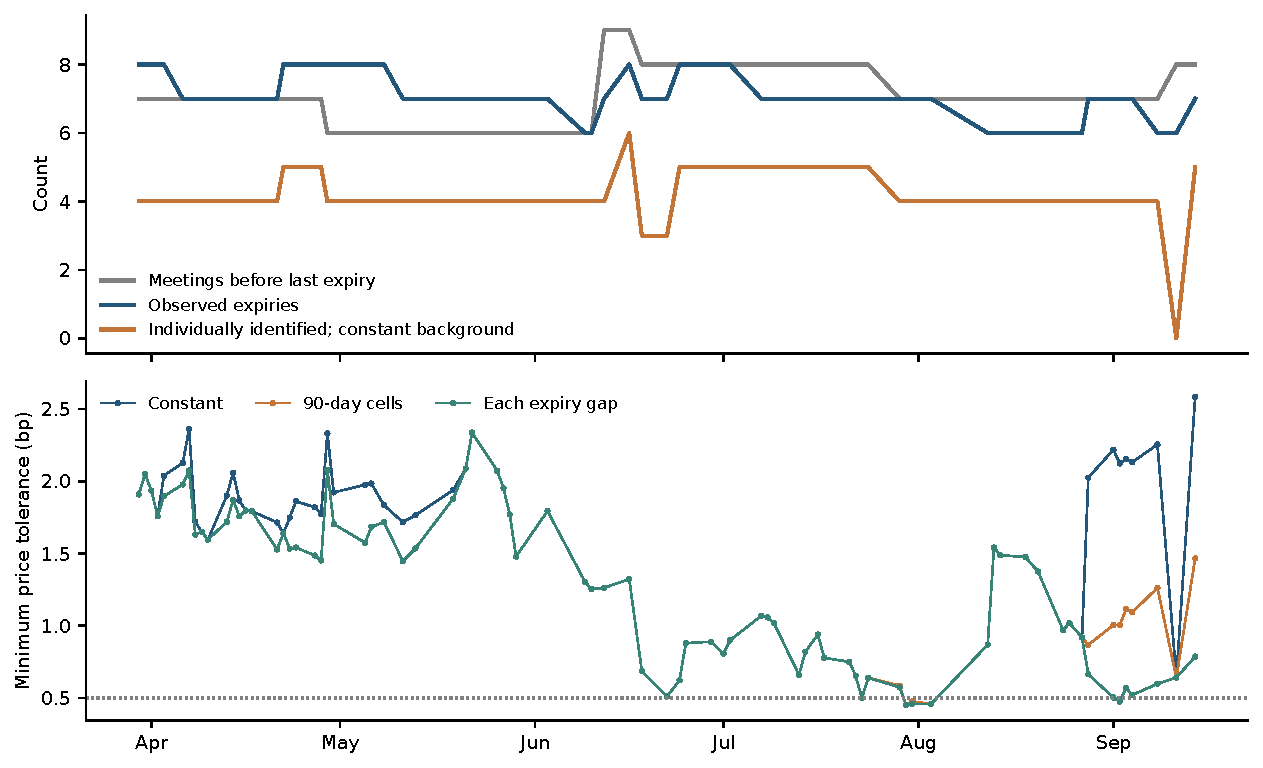
\includegraphics[width=.96\textwidth]{figures/empirical_calendar_fit.pdf}
\caption{Calendar information and price compatibility across the 78 observed dates. Top: numbers of meetings, expiries, and individually identified meeting variances under constant background. Bottom: the minimum premium tolerance needed to fit all selected out-of-the-money strikes under the discounted normal diagnostic. The dotted line is 0.5 bp. Lines connect the irregular observations; the contract set changes as expiries roll.}\label{fig:empiricalcalendar}
\end{figure}

Table~\ref{tab:empiricalfit} shows that calendar flexibility alone does not resolve the pricing problem. With constant background, only four dates fit at 0.5 bp and 23 fit at 1 bp. Even with a separate background rate in every expiry gap, only five dates fit at 0.5 bp. No specification fits any date at 0.25 bp. These are deterministic compatibility counts for this sample, not a statistical rejection frequency for the market population.

\begin{table}[ht]
\centering\small\begin{tabular}{lrrrr}\toprule Background variance & Median min. error & $\pm0.25$ & $\pm0.5$ & $\pm1$ \\\midrule
Constant & 1.683 & 0 & 4 & 23 \\
90-day cells & 1.449 & 0 & 4 & 24 \\
Each expiry gap & 1.411 & 0 & 5 & 30 \\
\bottomrule\end{tabular}

\caption{Minimum-error diagnostics and numbers of feasible dates out of 78. The second column is the median minimum tolerance, in premium bp; the remaining columns count dates fitting all selected strikes within the stated tolerance.}\label{tab:empiricalfit}
\end{table}

Using just the closest strike at each expiry makes the fit look substantially better. The median minimum tolerance falls from 1.683 to 0.247 bp for constant background. With an expiry-gap background, every date's closest-strike panel fits to within the numerical tolerance of 0.0001 bp. This is a weak fit test: any nondecreasing cumulative variance sequence can be reproduced with zero meeting variances by assigning each increment entirely to its gap's background rate. Yet the median minimum tolerance using all selected strikes remains 1.411 bp. A flexible variance schedule can reproduce these few inputs while missing the shape of the option prices.

\paragraph{Decomposing the fitting error.}
For each date, first allow each chain its own unrestricted normal variance and take the maximum of its chainwise minimum uniform errors. This is the smallest error possible before imposing any relation across expiries. Its median across dates is 1.411 bp, and it permits five dates at 0.5 bp and thirty at 1 bp. On all 78 dates, adding the expiry-gap model changes this benchmark by less than 0.000051 bp, below the bisection precision. The failure of that flexible specification is therefore already explained by within-chain pricing error. The calendar restrictions add no measurable minimum-error increment in this sample.

The standard sample has one retained chain per expiry on each date. Thus any additional cross-chain constraint combines expiry ordering with changing underlying quarters; these data cannot separate the two effects. The same-expiry midcurve experiment below tests the common-variance restriction across underlying quarters directly. Relative to the expiry-gap fit, constant background increases the required tolerance on 30 dates and 90-day background on nine dates, using 0.0002 bp to separate increases from numerical error. The largest constant-background increment is 1.799 bp. These additional errors arise from the variance specification, rather than additional smile error.

This conclusion is not driven solely by rows with no reported activity. As a separate screen, retain selected option sides with positive reported volume and open interest of at least 100. Each retained chain must still have at least three strikes in total, including strikes on both sides of the future. All 78 dates still have at least two chains. The median minimum tolerance with constant background is 1.410 bp. Reported activity is not a guarantee of executable liquidity, but this screen shows that the baseline discrepancy survives a simple activity restriction.

The baseline meeting-risk ranges and omitted-expiry checks are reported in Appendix~\ref{app:baseline}. The central sensitivity survives the better smile fit below: a positive meeting-risk lower bound can disappear when background variance is made more flexible.

\subsection{Same-expiry options on later futures}
Midcurves provide a different check. Under the parallel normal diagnostic, options with the same expiry have the same cumulative rate variance even when their underlying reference quarters differ. Apply the standard chain's closest-strike normal variance to a same-expiry midcurve, retaining the midcurve's own futures price, strike, and discount factor. The same chain-selection rule yields 165 comparisons on fourteen overlapping dates. The median absolute premium error is 3.438 bp and the maximum is 8.762 bp. The median midcurve-to-standard implied-standard-deviation ratios are 1.387 for S0, 1.221 for S2, and 1.225 for S3, based on 70, 58, and 37 comparisons respectively.



Ratios above one require larger terminal variance on the later windows under this diagnostic. The exponentially decaying loading in Section~\ref{sec:shape} predicts the opposite ordering for shifted equal-length windows: its averaged Brownian loading decreases with the window's start, while meeting loadings stay parallel. An increasing segment of a maturity-volatility curve, possibly followed by a hump, is therefore a relevant alternative; these ratios alone neither identify its shape nor distinguish it from smile and exercise effects. Section~\ref{sec:humpfit} fits such a shape, recomputes the exposures, and tests a withheld product.

The midcurve discrepancies are economically larger in premium units than many of the tolerance scenarios used to allocate meeting risk. They motivate testing maturity-dependent loadings and the listed exercise convention before using the parallel fit for relative value. They do not by themselves establish that midcurves are overpriced: the transported model has failed a pricing check.


\subsection{An at-the-money observation from a fitted smile}\label{sec:smileextension}
The within-chain errors need not be inherited by the calendar fit. We now fit a smile to each chain and use its interpolated at-the-money (ATM) price as the observation. An ATM smile estimate supplies a local variance proxy without integrating unobserved tails. It uses the same 555 standard chains and strike screen as the baseline.

Write the terminal futures-index displacement, in rate bp, as a mixture
\begin{equation}\label{eq:mixture}
I_S-I_0\ \sim\ \tfrac12 N(d,s_1^2)+\tfrac12 N(-d,s_2^2).
\end{equation}
The mean is fixed at the observed future. Each component has an elementary normal call formula, and their average gives a convex European price curve. Fit $d,s_1,s_2$ by unweighted least squares to the selected out-of-the-money settlements. Appendix~\ref{app:empiricalmethod} specifies bounds, starts, and convergence checks. The mixture is a price interpolant: it is not asserted to be the terminal law of the Gaussian rate model or a joint model across expiries.

Let $\widehat c_{\rm ATM}$ be its fitted ATM price and define
\begin{equation}\label{eq:smileatm}
\widehat{\cV}_{\rm ATM}=2\pi(\widehat c_{\rm ATM}/D)^2.
\end{equation}
This is the variance giving the same ATM premium in the normal formula. It is generally different from the mixture's second moment $d^2+(s_1^2+s_2^2)/2$. We apply the calendar matrix to this ATM proxy; its additivity is assessed in Section~\ref{sec:additivity}. For a sensitivity allowance $\varepsilon$ around the fitted ATM price, its interval is
\[
2\pi\{(\widehat c_{\rm ATM}-\varepsilon)^+/D\}^2
\ \leq\ \cV_{\rm ATM}\ \leq\
2\pi\{(\widehat c_{\rm ATM}+\varepsilon)/D\}^2.
\]
Write $\theta_{\rm ATM}$ for the nonnegative meeting and background parameters in the separate working equation $\boldsymbol{\cV}_{\rm ATM}=\mathsf A\theta_{\rm ATM}$. The endpoint programs are sharp conditional on these intervals and this additive ATM-variance schedule. The common empirical assumptions and interpretation of these sensitivity intervals are collected in Appendix~\ref{app:empiricalmethod}.

The median maximum strike error falls to \textbf{0.161 bp}, compared with 0.747 bp for the best one-variance normal fit; the largest mixture error is 0.918 bp. To test interpolation rather than only fit, remove the closest strike, refit, and predict that quote. Require at least five original strikes and observations on both sides after removal. This leaves 538 standard chains. Their median absolute held-out error is \textbf{0.124 bp}, and their maximum is 1.338 bp. These results support using the fitted ATM value as a local summary while showing that a quarter-basis-point allowance is not universally adequate.

\begin{table}[ht]
\centering\small
\begin{tabular}{lrrrr}
\toprule
Background & Median minimum (bp)& $0.25$ bp & $0.5$ bp & $1$ bp\\
\midrule
Constant &0.215&43&67&71\\
90-day cells &0.006&63&69&76\\
Each expiry gap &$<0.0001$&78&78&78\\
\bottomrule
\end{tabular}
\caption{Calendar compatibility of smile-fitted ATM observations. Counts are feasible dates out of 78. Tolerances surround fitted ATM premiums, so these counts are not directly comparable to the all-strike settlement counts in Table~\ref{tab:empiricalfit}.}\label{tab:smilefit}
\end{table}

All expiry-gap ATM panels are compatible to numerical precision. Thus the flexible calendar's failure in the baseline was not evidence against the ordering of cumulative ATM risk. Constant background still requires a median 0.215 bp allowance; additional background flexibility matters even after improving smile fit.

The meeting-risk bounds still depend on the background. On 18 June, using a 0.25 bp ATM-price allowance, the September meeting has range $[882,1080]$ bp$^2$ under constant background, $[807,1364]$ with 90-day cells, and $[0,1434]$ with expiry-gap cells. The January 2027 meeting has range $[2100,2507]$ under constant background and $[0,3371]$ under either flexible specification. Section~\ref{sec:exerciseempirical} repeats this comparison with wider expiry-specific allowances for exercise and mean effects.



A full European strip would instead identify a second moment. At pivot $x_0$, static payoff integration gives
\[
\frac2D\left\{\int_{-\infty}^{x_0}P_E(K)\,\dd K+
\int_{x_0}^{\infty}C_E(K)\,\dd K\right\}
=\Var^S(I_S)+(\E^S[I_S]-x_0)^2.
\]
It is a variance only at the expiry-forward mean. The American settlements and finite strike band here do not provide that strip: omitted tails have no finite upper bound without a tail assumption. The distinction is also relevant to the longer-sample short-rate uncertainty measure of \citet{bauer2021market}.

\subsection{Fitting a maturity loading and testing another window}\label{sec:humpfit}
Use the same smile procedure for the midcurves. First consider the bounded background loading
\begin{equation}\label{eq:humpshape}
\phi(s,T)=1+\chi\kappa(T-s)e^{-\kappa(T-s)},\qquad \chi\geq0,\quad\kappa>0.
\end{equation}
Its maximum is $1+\chi/e$ at distance $1/\kappa$, and it returns to one at long maturities. Meeting loadings remain parallel. For each shape, average the loading over each contract's window and compute the background exposures in \eqref{eq:shapeD}. We fit this matrix to the ATM proxy; Appendix~\ref{app:empiricalmethod} gives the numerical procedure and its assumptions.

There are fourteen dates with standard and same-expiry midcurve observations. Fit the common shape using the 219 standard, S0, and S2 observations, with date-specific nonnegative meeting variances and one background rate. For each candidate, solve weighted nonnegative least squares in variance, with weights $1/(2\sqrt{\widehat{\cV}_{\rm ATM}})$, then select the smallest actual standard-deviation RMSE. The original grid has $\chi\in\{0,0.5,1,2,4,8\}$ and $\kappa\in\{0.25,0.5,0.75,1,1.5,2,3\}$ year$^{-1}$: 42 parameter pairs but 37 distinct shapes. It selects $(\chi,\kappa)=(4,0.75)$. Training RMSE falls from 5.406 to 1.417 bp, while the mean absolute error on the 37 unused S3 observations rises from 1.706 to 3.818 bp.

The return to one may be too restrictive: the observed S2 and S3 volatility ratios both exceed one. We therefore add a long-end level,
\begin{equation}\label{eq:levelshape}
\phi(s,T)=1+\chi_1\kappa(T-s)e^{-\kappa(T-s)}
               +\chi_2(1-e^{-\kappa(T-s)}),\qquad \chi_1,\chi_2\geq0.
\end{equation}
This loading remains positive and bounded, with limit $1+\chi_2$. The grid in Appendix~\ref{app:empiricalmethod} has 496 distinct shapes and selects $(\chi_1,\chi_2,\kappa)=(12,8,1.5)$. Selection and date-specific fitting again use only the 219 training observations. Since $\chi_2=8$ is the primary grid's upper limit, we repeat selection on a 1,081-shape grid extending both amplitudes to 64. The same shape wins. Expanding the pure-hump subgrid to 64 distinct shapes also leaves its original optimum unchanged.

\begin{table}[ht]
\centering\small
\begin{tabular}{lrr}
\toprule
Background loading & Training SD RMSE (bp) & S3 SD MAE (bp)\\
\midrule
Parallel & 5.406 & 1.706\\
Hump returning to one & 1.417 & 3.818\\
Hump with free long-end level & 1.148 & 1.131\\
\bottomrule
\end{tabular}
\caption{Same-date product prediction: 219 standard/S0/S2 training observations and 37 S3 observations on fourteen dates. All parameter choices minimize training error. The additional family was proposed after examining the original S3 failure, so its result is a diagnostic reuse of that sample.}\label{tab:loadingcomparison}
\end{table}

Allowing the long-end level reduces S3 mean absolute error to 1.131 bp (median 1.047 bp), below both earlier specifications. Thus the original negative result is partly specific to the loading family; it does not by itself reject a common maturity loading. Figure~\ref{fig:extensions} shows where the products fall on the two selected shapes. The curves are normalized at one year because the fitted background scale absorbs their absolute level. The selected loading is 0.089 of its one-year value at zero maturity distance and 0.843 at half a year. Economically, it assigns little non-meeting volatility to the nearest forwards, consistent with a front end anchored by policy meetings. This interpretation depends on separating meeting and background risk as specified. Flattening the first half-year of the loading leaves the 22 July expiry-gap matrix rank at 12 of 15, but reduces its smallest nonzero singular value relative to its largest by a factor of 5.3. Thus exact rank does not capture how strongly the steep front distinguishes background exposures. Appendix~\ref{app:finalsensitivities} gives this controlled perturbation without refitting the model.

\begin{figure}[ht]
\centering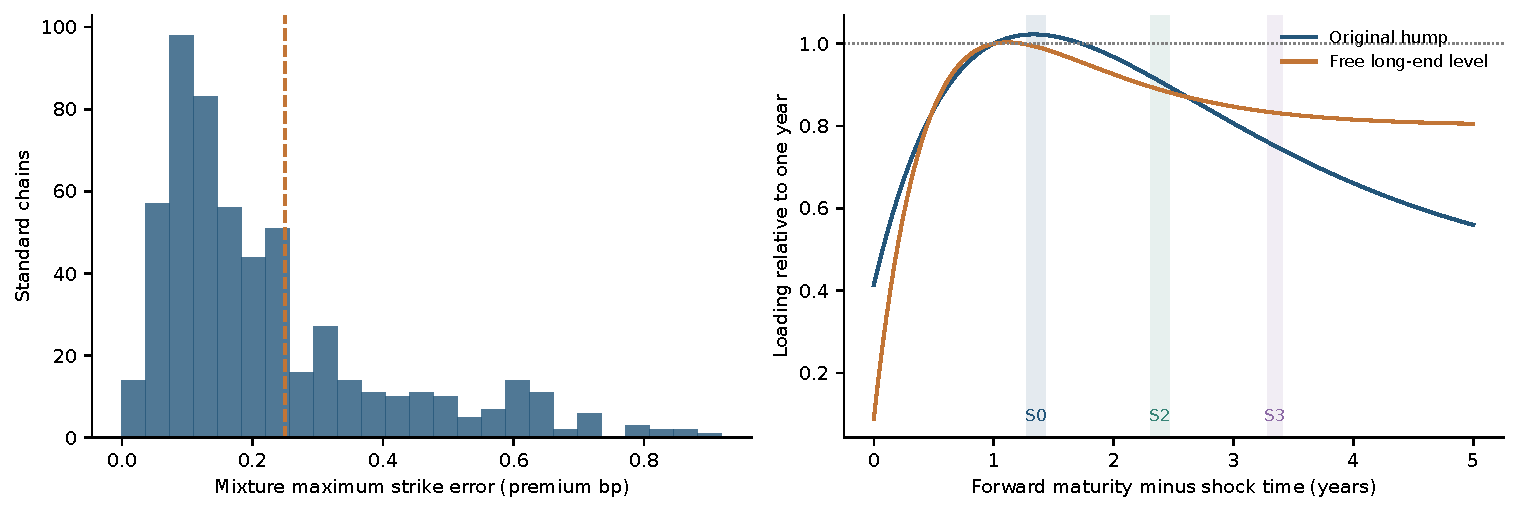
\includegraphics[width=\textwidth]{figures/empirical_extensions.pdf}
\caption{Extensions using the existing public settlements. Left: maximum selected-strike error in each standard chain's normal-mixture fit; the dashed line is 0.25 bp. Right: the two background loadings selected using standard, S0, and S2 observations, each divided by its value at one year. Shaded bands show the interquartile ranges of representative maturity distances $(a+b)/2-S/2$ for S0, S2, and S3. The exposure calculation integrates over the full accrual window and shock-time interval, not just these representative positions.}\label{fig:extensions}
\end{figure}

Each S3 exposure row lies in the span of its date's training rows, to numerical precision. Nonuniqueness of meeting allocations therefore does not alter the prediction conditional on the fitted training rows. These are point predictions, not bounds over price intervals. The new family was motivated by the earlier S3 errors; an untouched product or later sample is needed for independent validation of that family. Appendix~\ref{app:shapeprofile} retains the original-hump interval and shape-profile calculations, which show how shape uncertainty widens meeting-risk ranges.

\subsection{How large are exercise and mean adjustments?}\label{sec:exerciseempirical}
For an exercise benchmark, let the futures index be an arithmetic Brownian martingale with constant variance rate calibrated to the chain's fitted ATM variance. Discount at the constant rate reproducing its observed $D$. Value cash exercise on a recombining trinomial tree with 400, 800, and 1,600 time steps. Exercise is allowed at every step. Subtract the European value on the \emph{same} tree to isolate early exercise from terminal-payoff discretization. Appendix~\ref{app:empiricalmethod} specifies the tree and its pricing assumptions.

Use the first, middle, and last sample dates (30 March, 16 June, 14 September), and each chain's closest strike and two strike-band endpoints: 69 option observations. The 1,600-step exercise premium has median \textbf{0.023 bp} and maximum \textbf{0.377 bp}. The maximum change from 800 to 1,600 steps is 0.00050 bp; the largest European-tree error against the analytic normal price is 0.0034 bp. The largest exercise premium is for the 10 September 2027 expiry observed on 14 September 2026. Exercise is small for the median selected quote but material relative to a 0.25 bp allowance for some long expiries. It is too small in this benchmark to explain the multi-basis-point median midcurve error by itself. 

The mean effect can be sized without an exercise solver. Conditional on the 18 June ATM-proxy intervals at 1 bp, optimize the linear row $z/\delta$ in \eqref{eq:zrows}. For this sensitivity calculation only, insert those bp$^2$ allocations into the Gaussian model, converting variance to decimal units. The rate-mean displacement is
\[
F_0-\E^S[F_S]=\frac{G_0(1-e^{-z})}{\delta}.
\]
Across the three background specifications its compatible range is about $[0.00049,0.00096]$ rate bp for the first expiry and $[0.298,0.445]$ bp for the last, 11 June 2027. This is a conditional scale calculation, not a simultaneous fit of the exact cash means and variances. At fixed log variance, a European call or put price is Lipschitz in its rate mean with constant at most $D$. Hence the corresponding premium change is at most $D$ times the reported mean displacement. The longest expiries can require a wider allowance even when the smile interpolation itself is accurate.

We now widen the 18 June ATM-price allowances by both benchmark effects:
\begin{equation}\label{eq:robustallowance}
\varepsilon_\ell=0.25+\widehat{\mathrm{EEP}}_\ell
                         +D_\ell\overline{\Delta m}_\ell\quad\text{premium bp}.
\end{equation}
Here $\widehat{\mathrm{EEP}}_\ell$ is the 1,600-step exercise premium evaluated at the fitted ATM variance and zero moneyness. The mean bound $\overline{\Delta m}_\ell$ is the largest upper displacement across the three background specifications, each computed from its 1 bp seed intervals. This gives the same allowance for all three comparisons. The resulting allowances range from 0.253 to 0.989 bp across the seven expiries. Every allowance remains below 1 bp, so each new feasible set lies within the seed set used to bound its mean adjustment. The largest 800-to-1,600-step exercise change is 0.000033 bp.

\begin{table}[ht]
\centering\small
\begin{tabular}{lrr}
\toprule
Background & 16 September 2026 & 27 January 2027\\
\midrule
Constant & $[858,1100]$ & $[1910,2696]$\\
90-day cells & $[754,1384]$ & $[0,3560]$\\
Each expiry gap & $[0,1456]$ & $[0,3560]$\\
\bottomrule
\end{tabular}
\caption{18 June meeting-variance ranges in bp$^2$ with the expiry-specific allowances \eqref{eq:robustallowance}. Endpoints are rounded to the nearest bp$^2$.}\label{tab:robustranges}
\end{table}

The positive constant-background lower bounds survive (Table~\ref{tab:robustranges}). Relative to the 0.25 bp calculation, January's lower bound falls from 2,100 to 1,910 bp$^2$; allowing a flexible background still reduces it to zero. This establishes sensitivity to the background even after the specified exercise and mean allowances. The exercise estimate is a normal-model benchmark, not a uniform upper bound for every American model; the mean bound is conditional on inserting the proxy allocations into the Gaussian model.

\subsection{Does an ATM variance add across discrete meetings?}\label{sec:additivity}
A good smile interpolation does not guarantee an additive variance observation. For a centred terminal displacement $X$, the ATM proxy is $(\pi/2)(\E|X|)^2$. Independent Gaussian increments make it additive, but independent discrete increments generally do not. Consider equal-probability jumps of $\pm25$ bp. One jump and the sum of two such jumps both have $\E|X|=25$ bp, so both have ATM variance $625\pi/2=981.75$ bp$^2$, although their true variances are 625 and 1,250 bp$^2$. Adding two one-meeting ATM proxies overprices the two-meeting ATM call by 5.126 bp when the meetings are at $1/8$ and $2/8$ year and discounting is at 4\%.

Adding independent Gaussian background moderates the error but need not reduce it below 0.25 bp. With background volatility 50 bp per square-root year, eight equally spaced meetings produce a maximum ATM-price discrepancy of 2.323 bp from the additive one-increment proxy. If instead the additive schedule is allowed to fit each expiry exactly, its implied meeting variances range from 549 to 770 bp$^2$, despite all true meeting variances being 625 bp$^2$. The largest allocation errors occur at the first two meetings (770 and 549 bp$^2$); by the third, the inferred variance is 633 bp$^2$. In this example the error is concentrated where little background risk has accumulated, precisely the nearest meetings that front-end users often want to isolate. Appendix~\ref{app:additivity} gives the exact calculation and further background levels. The exercise-and-mean allowances above do not address this structural proxy error. The empirical ranges identify allocations within the additive ATM specification; interpreting them as variances of discrete policy outcomes requires a distributional pricing model or an additional sensitivity analysis.

Actual variance is additive across independent increments under a common measure, regardless of their distribution. As a companion check, Appendix~\ref{app:finalsensitivities} uses the fitted mixture second moments for the 18 June panel. This replaces the nonlinear ATM transform but introduces tail extrapolation. With the same ATM-scale perturbations and an additional 10\% moment allowance, constant-background September and January ranges are $[275,1058]$ and $[1549,4229]$ bp$^2$; both flexible backgrounds allow zero for both meetings. At 25\%, September's constant-background lower bound also vanishes and January's falls to 91 bp$^2$; at 50\%, both vanish. Without the additional allowance, constant and 90-day backgrounds are infeasible. Thus the background contrast appears under both proxies at a stated sensitivity level, but positive lower bounds are not robust to arbitrary tail uncertainty.


\FloatBarrier
\section{Possible uses in trading and risk management}\label{sec:uses}
The analysis is most useful before a trader turns a fitted meeting variance into a position. It distinguishes a price disagreement that survives model uncertainty from one created by a chosen background schedule or maturity loading. The examples below concern valuation screens and exposure construction. The settlement panel does not establish an executable profit or a realized hedging advantage.

\subsection{Event-volatility calendar spreads}
An option expiring before a meeting and one expiring after it have different event exposures. Their variance difference also contains the ordinary volatility accumulated between the two expiries. A calendar spread therefore needs weights chosen for the risk one wants to remove; one contract against one contract generally leaves background exposure.

Here is a local construction in the normal diagnostic, keeping the futures index and discount factors fixed when differentiating variances. Consider two straddles on the same underlying future, where a straddle is one call plus one put at a common strike. Let $S_1<S_2$ be their times to expiry, let $\cV_{\mathrm N,j}>0$ be their inferred normal variances, and let $D_j$ and $x_j$ be their discount factors and absolute moneyness in rate bp. Their sensitivities to cumulative variance are
\[
g_j=\frac{D_j\varphi(x_j/\sqrt{\cV_{\mathrm N,j}})}{\sqrt{\cV_{\mathrm N,j}}},\qquad j=1,2.
\]
With constant background variance rate $u$, the sensitivity to $u$ is $g_jS_j$. A position of one later straddle and
\begin{equation}\label{eq:calendarhedge}
-\frac{g_2S_2}{g_1S_1}
\end{equation}
earlier straddles has zero first-order background sensitivity at the calibration point. A meeting strictly between the expiries enters only the later variance, so its sensitivity is $g_2$. A meeting before the first expiry enters both legs and has net sensitivity $g_2(1-S_2/S_1)$, which is negative. The position therefore retains earlier-meeting exposure; cancelling background variance does not isolate a single event. Delta can be offset with the underlying future. This is a local hedge: the weights change with prices and time, and the earlier option expires before the event. It is not a static replication of an event-variance payoff. A multidimensional background generally requires more option legs and enough independent sensitivities.

On 14 September, the selected October 16 and November 13 options both reference the December 2026 future. Their closest common strike is 95.75, and the October 28 meeting lies between their expiries. The September 16 meeting precedes both expiries. The calculation gives one November straddle against 1.388 October straddles sold. Under the same diagnostic, their combined delta is offset by buying approximately 0.0117 December futures per November straddle. Per unit increase of one bp$^2$ in a meeting variance, the local premium sensitivities are approximately $+0.01337$ bp for October 28 and $-0.01170$ bp for September 16. These fractional ratios and sensitivities describe exposure per unit position; any actual implementation needs feasible sizes and sensitivities computed with a listed-option pricer. They are calculated from separate closest-strike implied variances, without claiming that the full September 14 surface fits the diagnostic.

The construction specifies what the position is exposed to, not why it should earn money. A relative-value screen should first withhold the proposed trade's quotes, calibrate to other contracts, and optimize its value over the compatible allocations. The omitted-expiry exercise in Appendix~\ref{app:baseline} is a simple version of that screen and finds no out-of-range quote interval on its feasible dates. Calling the midcurve discrepancies a trade would be premature because the transported model already misses those prices systematically. For a multi-leg position, optimize the portfolio's value jointly; combining marginal upper and lower bounds can select allocations that cannot coexist.

\subsection{Futures against an OIS forward}
The data also permit a direct comparison of futures rates with discount-curve forwards. For a reference quarter $[a,b]$ of ACT/360 length $\delta$, the forward rate implied by a SOFR discount curve is
\begin{equation}\label{eq:oisforward}
\frac{P(0,a)/P(0,b)-1}{\delta}.
\end{equation}
This is the par rate of an ideal single-period compounded swap paid at $b$, not the par coupon of a longer multi-payment OIS. Payment delays and other actual swap conventions must be matched before constructing a hedge.

In the model of Proposition~\ref{prop:pricing}, $P(0,a)/P(0,b)=e^{A_0}$ and the rate futures is $(e^{A_0+p}-1)/\delta$. Their difference is therefore
\begin{equation}\label{eq:convexitygap}
\frac{e^{A_0}(e^p-1)}{\delta}.
\end{equation}
The exponent $p$ weights meeting and background variances through the end of accrual. An option panel ending earlier need not determine all of those contributions. A defensible screen retains the unobserved tail risks. If an unconstrained meeting or background contribution after the last observed expiry enters $p$ with positive weight, its convexity upper bound is infinite. A finite upper bound then requires an additional observation or an explicit tail restriction; it cannot be obtained by silently extending the fitted background. Futures--swap comparisons and their convexity adjustments are established applications; here the additional question is how much the proposed adjustment depends on an unidentified variance allocation. See \citet{skov2021dynamic} for SOFR futures pricing and convexity adjustments.

For each distinct date and underlying reference quarter represented by a standard option with 7--365 days to expiry, compare the observed SR3 futures rate with \eqref{eq:oisforward} from the same-date Eris curve. Deduplicating underlying quarters gives 309 observations. The median gap is 0.051 bp, with an interquartile range of $[0.011,0.249]$ bp and a full range of $[-1.737,1.988]$ bp. Fifty-six gaps are negative.

\begin{figure}[ht]
\centering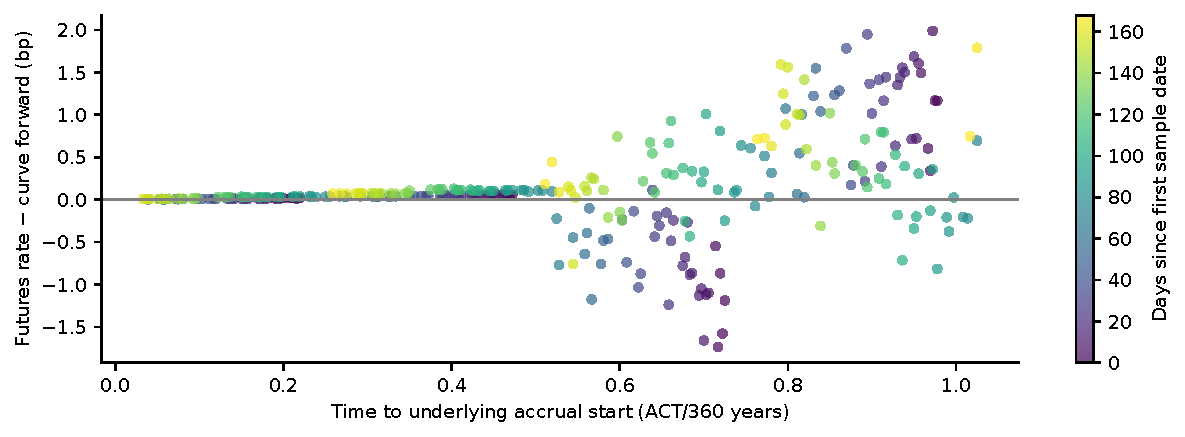
\includegraphics[width=.96\textwidth]{figures/empirical_convexity.pdf}
\caption{Observed SOFR futures rate minus the same-window forward rate from the Eris curve, in rate bp. Each point is a distinct date and underlying reference quarter. These are curve comparisons before any model convexity adjustment, execution costs, or intraday synchronization correction.}\label{fig:empiricalconvexity}
\end{figure}

Under the ideal Gaussian model, $p\geq0$, so a negative exact gap is incompatible with treating those inputs as a common exact model observation. It does not establish a tradable arbitrage in these datasets. Eris supplies a constructed curve, the observations are not synchronized executable quotes, and the traded swap's conventions may differ from \eqref{eq:oisforward}. The small median gap makes those distinctions consequential. A candidate trade would require an independently quoted, convention-matched OIS and an offsetting futures strip, with the residual outside the full adjustment and cost range. CME Clearing Advisory 23-050 specifies one monthly SOFR future and up to thirteen quarterly SOFR futures, alongside Eris swap futures and SOFR OIS, as inputs to the published Eris SOFR curve.\footnote{CME Clearing, 14 February 2023, effective 27 February 2023: \url{https://www.cmegroup.com/notices/clearing/2023/02/Chadv23-050.pdf}.} All 309 compared quarters start within 1.03 years, inside that maximum futures-input horizon. The public daily discount factors do not disclose the constituent set, fitting weights, or curve sensitivities, so an SR3 percentage contribution cannot be recovered from them. The documented input overlap is sufficient to rule out interpreting these small gaps as an independent market test of futures convexity.


\FloatBarrier
\section{Conclusion}
Meeting-risk calibration is subject to two different constraints: what prices distinguish and what a model permits. In the Gaussian model, post-cutoff cash claims retain only total earlier variance, even with continuous background risk and American exercise. Later-accruing futures retain its first time moment as well. Earlier expiries can separate more of the allocation, according to the rank of their meeting and background exposures; finite premium precision determines whether that separation is useful.

For scheduled-rate factor models, arbitrary deterministic scale recalibration leaves a finite variance cone. Under constant ordinal loadings, its complete restrictions are consecutive-meeting inequalities. With square-root stochastic volatility, the full drift-and-leverage kernel gives an affine variance map whose exact support and covariance rank depend on the active variance states. The two published three-factor specifications consequently impose different numbers of affine restrictions. These conclusions concern model restrictions, independently of whether a particular option panel identifies the underlying meeting variances.

The settlement application shows why both distinctions belong in a calibration report. A smile fit sharply reduces pricing errors, yet changing the background still removes positive meeting-risk lower bounds. A known nonparallel loading lets same-expiry options on different futures add information; estimating that loading creates another source of uncertainty. Allowing a free long-end loading improves three-year-midcurve predictions relative to a hump returning to one, although the additional family still needs an untouched validation sample. Positive constant-background bounds survive expiry-specific exercise and mean allowances. In the discrete-outcome example, ATM-variance additivity can fail by much more than those allowances; good interpolation alone cannot establish structural meeting variances. Fitted second moments retain the constant-versus-flexible contrast with a 10\% extra moment allowance, but wider extrapolation bands remove the positive lower bounds. The two proxies expose different sources of uncertainty in the allocation.

A useful calibration therefore reports compatible meeting and group ranges alongside the restrictions used to obtain them. It tests withheld contracts and distinguishes a better fit from better predictions. The theoretical price-equivalence and factor-support results explain why some ambiguities persist even with richer pricing, while the numerical analysis shows where stronger modelling assumptions are doing the work.

\appendix
\section{Proofs}
\subsection{Bond and option pricing}\label{app:pricing}
\begin{proof}[Proof of Proposition~\ref{prop:bond}]
Integration of \eqref{eq:curve}, followed by deterministic and stochastic Fubini, gives
\begin{align}\label{eq:discountbond}
\frac{P(t,T)}{B_t}=P(0,T)&\exp\left\{-\int_0^t(T-s)\sigma(s)\,\dd W_s
                        -\frac12\int_0^t(T-s)^2\sigma(s)^2\,\dd s\right\}\nonumber\\
&\times\prod_{T_i\leq t}\exp\{- (T-T_i)X_i-\tfrac12(T-T_i)^2v_i\}.
\end{align}
All deterministic integrands are bounded on the finite horizon. The Brownian factor is a true exponential martingale. Each meeting factor has conditional expectation one when it is revealed, since $X_i$ is an independent centred Gaussian of variance $v_i$. Brownian increments and unrevealed meeting variables are jointly independent of the past. Conditioning the product between any two times therefore preserves its value. It is integrable with expectation $P(0,T)$ and is a true martingale. Since $P(T,T)=1$, conditioning its terminal value gives the stated bond valuation identity.
\end{proof}

\begin{proof}[Proof of Proposition~\ref{prop:pricing}]
Write
\[
L_t=\sum_{T_i\leq t}w(T_i)X_i+\int_0^t\sigma(s)w(s)\,\dd W_s,\qquad
q_t=\sum_{T_i\leq t}w(T_i)^2v_i+\int_0^t\sigma(s)^2w(s)^2\,\dd s
\]
for $0\leq t\leq b$. Integrating the short rate over $[a,b]$ yields
\[
\log R(a,b)=A_0+L_b+\sum_i d(T_i)v_i+\int_0^b\sigma(s)^2d(s)\,\dd s.
\]
The unrevealed portion of $L_b$ is independent centred Gaussian with variance $q_b-q_t$. Taking its exponential expectation gives
\begin{equation}\label{eq:Gmart}
G_t=\exp\{A_0+p+L_t-q_t/2\}.
\end{equation}
This also proves integrability and the martingale property of $G$.

At time $S$, Proposition~\ref{prop:bond} shows that $B_S^{-1}/P(0,S)$ is a probability density. Its random logarithm has coefficients $-(S-T_i)$ on $X_i$ for $T_i\leq S$, and $-(S-s)\sigma(s)$ on Brownian increments. Exponential tilting of a jointly Gaussian vector shifts the mean of $L_S$ by $\Cov(L_S,\log B_S^{-1})=-z$ and leaves its variance $q=q_S$ unchanged. Consequently $\log G_S$ under this density has law
\[
N(\log G_0-z-q/2,\ q).
\]
Integrating $(G_S-K)^+$ gives \eqref{eq:price} and \eqref{eq:black}, including the deterministic limit at $q=0$.

For completeness, the complete positive-strike surface recovers its parameters without presuming that they are already known. Because $G_S>0$ almost surely,
\[
\lim_{K\downarrow0}\frac{C(S,K)-C(S,0)}{K}=-P(0,S),\qquad
C(S,0):=\lim_{K\downarrow0}C(S,K)=P(0,S)m.
\]
The first equality follows by dominated convergence from the difference quotient of the call payoff, which is bounded between $-1$ and zero. The second follows by monotone convergence or integrability. Thus the surface determines $P(0,S)$ and $m$. At strike $K=m$,
\[
\frac{C(S,m)}{P(0,S)m}=2\Phi(\sqrt q/2)-1,
\]
which is strictly increasing from zero to one as $q$ ranges from zero to infinity. This determines $q$. The formulas for $z$ and $p$ then follow from $m=G_0e^{-z}$ and $G_0=e^{A_0+p}$. For $S<a$, $w=\delta$ on $[0,S]$. Fubini in \eqref{eq:Q} gives $\int_0^S\cV(x)\,\dd x=\sum_{T_i\leq S}(S-T_i)v_i+\int_0^S(S-s)\sigma(s)^2\,\dd s$, proving \eqref{eq:Qz}.
\end{proof}

\paragraph{The maturity-dependent extension.}
Let $\Psi(s,T)=\int_s^T\phi(s,x)\,\dd x$. For the curve in \eqref{eq:shapecurve}, the continuous discounted-bond factor in \eqref{eq:discountbond} becomes
\[
\exp\left\{-\int_0^t\sigma(s)\Psi(s,T)\,\dd W_s
            -\tfrac12\int_0^t\sigma(s)^2\Psi(s,T)^2\,\dd s\right\}.
\]
Indeed, $\int_s^T\phi(s,x)\Psi(s,x)\,\dd x=\Psi(s,T)^2/2$, since $\Psi(s,\cdot)$ is absolutely continuous. Boundedness ensures square integrability and permits stochastic Fubini, with a jointly measurable version. Integrating the short rate over $[a_\ell,b_\ell]$ gives the Brownian weight $\int_{a_\ell}^{b_\ell}\phi(s,x)\,\dd x=\delta_\ell\beta_\ell(s)$ for $s\leq S_\ell<a_\ell$. Gaussian conditioning and discount tilting preserve its variance. Dividing that variance by $\delta_\ell^2$ proves \eqref{eq:shapeD}. This argument supplies the required normalized variance formula; the special time-integral identity for $z$ in \eqref{eq:Qz} need not survive a change in $\phi$.

\subsection{Rank and identified linear quantities}\label{app:rank}
\begin{proof}[Proof of Theorem~\ref{thm:rank} and Corollary~\ref{cor:shape}]
Use the general matrix with meeting columns $\ind_{\{T_i\leq S_\ell\}}$ and background columns $\mathsf D_{\ell j}$. Invertible row differencing, with a zero initial row, changes its $\ell$th row to
\[
\left((\ind_{\{S_{\ell-1}<T_i\leq S_\ell\}})_{i=1}^N,
                                  (\Delta \mathsf D_{\ell j})_{j=1}^{n_b}\right).
\]
A meeting later than $S_L$ has a zero column. Two meetings in the same gap have identical columns. Either event prevents full column rank.

Suppose every meeting is covered and no gap contains two meetings. A vector $(x,y)\in\R^N\times\R^{n_b}$ lies in the kernel if and only if, on each meeting-free gap, $\Delta \mathsf D_{\ell,\cdot}y=0$, and on the gap containing meeting $i$, $x_i=-\Delta \mathsf D_{\ell,\cdot}y$. If the meeting-free block has full column rank, the first equations force $y=0$ and the second force $x=0$. If it does not, choose a nonzero $y$ in its kernel and define each $x_i$ by the second equations. This gives a nonzero kernel vector of the full matrix. The rank criterion follows. The parallel case has $\mathsf D_{\ell j}=\mathfrak l_j((0,S_\ell])$ and $\Delta \mathsf D_{\ell j}=\mathfrak l_j((S_{\ell-1},S_\ell])$.

Full column rank implies injectivity on every subset. Conversely, let $d\ne0$ lie in the kernel and let $\theta$ be strictly positive. For sufficiently small nonzero real $\epsilon$, both $\theta$ and $\theta+\epsilon d$ are strictly positive and give the same observations. This proves failure of injectivity on the orthant and the stated interior conclusion.
\end{proof}

The linear-functional claim follows from the same argument. If $c=\mathsf A^\top a$, then $c^\top\theta=a^\top\boldsymbol{\cV}$ is determined. If $c$ is outside the row space, the identity $\row(\mathsf A)=(\ker\mathsf A)^\perp$ gives a $d\in\ker\mathsf A$ with $c^\top d\ne0$. Perturbing any positive $\theta$ along $d$ changes the functional while preserving the panel. This is an elementary finite-dimensional statement and requires no stochastic assumptions.

\subsection{Aggregation and the compatible polytope}\label{app:aggregation}
\begin{proof}[Proof of Theorem~\ref{thm:aggregate}]
In the pure-jump model,
\[
y=\sum_{i\leq k}(X_i+v_i (A-T_i)),\qquad
B_A^{-1}=\exp\left\{-\sum_{i\leq k}((A-T_i)X_i+\tfrac12v_i (A-T_i)^2)\right\}.
\]
The Gaussian exponential formula gives $\E[B_A^{-1}]=1$. Under this density the early coordinates are independent $N(-v_i (A-T_i),v_i)$ variables, and the later coordinates retain their independent $N(0,v_i)$ laws. Hence $y\sim N(0,V)$ and is independent of the later coordinates. Substitution in the forward curve gives \eqref{eq:postcurve}. Every post-$A$ bond, bank-account ratio, and bond-implied fixing is a fixed function of $y$, the later coordinates, and the total $V$.

Let $Y_S$ be the cash flow in part 2. Factor its discount as $B_S^{-1}=B_A^{-1}\exp(-\int_A^S r_t\,\dd t)$. Under the tilted measure, its value is an expectation of a fixed function of $y$ and the later coordinates. Their joint law depends on the early variances only through $V$. This proves the European assertion under the stated integrability assumption.

For American exercise, first assume $V>0$ and define early residuals
\[
\epsilon_i=X_i+v_i (A-T_i)-\frac{v_i}{V}y,\qquad i\leq k.
\]
Under the tilted measure, their covariances with $y$ are zero, and their covariances with every later coordinate are zero. Joint Gaussianity implies independence of the residual vector from $(y,X_{k+1},\ldots,X_N)$. Also the early information is exactly the information generated by $y$ and the residuals, since the displayed formula can be inverted. First restrict exercise to a finite deterministic grid containing $A$ and $S$. On the canonical product space, the sections of each full-history stopping event, after fixing the residual vector, are measurable in the reduced history generated by $y$ and the later coordinates revealed by that grid time. For almost every residual value, the resulting events define a reduced stopping rule. Completed filtrations cause no difficulty on a finite grid: choose raw measurable representatives of its finitely many stopping events, modifying them on a common null set if needed. Each section has expected reward at most the supremum over reduced grid stopping rules. Independence and Fubini give the same bound after averaging over residuals. The reverse inequality holds because every reduced rule is a full-history rule. The grid suprema are therefore equal.

For any full-history stopping time $\tau$, round it upwards to the next point of a sequence of nested grids with mesh tending to zero, retaining $S$ as an endpoint. The rounded time $\tau_n$ is a grid stopping time and decreases to $\tau$. Right continuity gives $\widehat Y_{\tau_n}\to \widehat Y_\tau$, and the integrable envelope gives convergence of expectations under the tilted measure. Thus the supremum over all stopping times is the limit of the grid suprema. The same argument applies to the reduced filtration, proving equality for continuous exercise. The reduced state law and payoff rule depend on the earlier variances only through $V$. If $V=0$, all early variances and variables vanish and no residual information is present. This proves part 3 without a claim that the optimal stopping time is an expiry time or even that an optimum is attained.

For part 4, when $T_i\leq A\leq a$, the weight in \eqref{eq:p} is $h(T_i)=\delta(b-T_i)$. Summing these contributions yields $\delta(bV-M_1)$. All later-meeting terms are held fixed. If two windows have distinct terminal dates $b_1,b_2$, subtract their known contributions and divide each logarithmic futures quote by its own $\delta$. The resulting values are $b_1V-M_1$ and $b_2V-M_1$, which determine $V$ and $M_1$ uniquely.
\end{proof}

For the polytope, divide \eqref{eq:polytope}'s second equation by $V>0$. The ratio $M_1/V$ is a convex combination of the meeting dates. This gives the feasibility criterion, whose converse follows by mixing the first and last dates. Compactness follows from $0\leq x_i\leq V$. If a feasible vector has at least three positive coordinates, the corresponding two-row matrix, whose columns are $(1,T_i)^\top$, has a nonzero kernel vector supported on those coordinates. A sufficiently small perturbation in either direction remains feasible and nonnegative. The original vector is not an extreme point. A linear objective on a nonempty compact polytope attains its extrema at extreme points; these therefore have at most two positive coordinates. Solving the two equations gives \eqref{eq:vertices}.

\subsection{Interval inversion and cumulative bounds}
Strict monotonicity of \eqref{eq:atm} and algebra give \eqref{eq:inverse}. Differentiating for $\cV>0$ gives
\[
\frac{\partial c}{\partial \cV}=\frac{Dm}{2\sqrt{\cV}}
                         \varphi(\delta\sqrt{\cV}/2),
\]
which proves the local relation \eqref{eq:eta}. For a linear estimator, its error is $a^\top e$. On the box $|e_\ell|\leq\eta_\ell$, its maximum absolute value is $\sum|a_\ell|\eta_\ell$, attained by aligning the error signs. Applying this to the coefficients of the differenced estimator proves \eqref{eq:differror}.

\begin{proof}[Proof of Proposition~\ref{prop:cumulative}]
Any feasible cumulative vector is nondecreasing. Hence $\cV_n\geq\max_{i\leq n}\ell_i=L_n$ and $\cV_n\leq\min_{j\geq n}r_j=R_n$. These inequalities imply necessity. Conversely, if $L_n\leq R_n$ for every $n$, the nondecreasing choice $\cV_n=L_n$ satisfies every original interval and proves feasibility.

For any consecutive pair, $\cV_{n-1}\geq L_{n-1}$ and $\cV_n\leq R_n$ give the upper bound in \eqref{eq:cumbounds}. Also $\cV_n\geq L_n$ and $\cV_{n-1}\leq R_{n-1}$ give its lower bound, together with nonnegativity. To attain the upper bound, set $\cV_{n-1}=L_{n-1}$ and $\cV_n=R_n$. Fill earlier coordinates with $L_j$ and later coordinates with $\max\{L_j,R_n\}$. For $j>n$, $R_j\geq R_n$, so these choices remain within their effective intervals and are nondecreasing.

For the lower bound, if $L_n>R_{n-1}$, choose the pair $(R_{n-1},L_n)$. Otherwise choose both coordinates equal to $\max\{L_{n-1},L_n\}=L_n$, which belongs to both effective intervals because $L_n\leq R_{n-1}\leq R_n$. Fill earlier coordinates with their lower envelopes and later coordinates with the maximum of their lower envelope and the chosen $\cV_n$. All interval and monotonicity constraints hold. For $n=1$, use the fixed value $\cV_0=0$, giving the same formulas. This proves sharpness.
\end{proof}

\section{Factor-model specification and support proofs}\label{app:support}
\subsection{The full conditional-variance map}\label{app:svderivation}
Put $\Gamma_{i,j}=\sum_{h=1}^i\gamma_{h,j}$, $\Gamma_{0,j}=0$, and
\[
h_j(s,T)=a_j(s)e^{-\kappa_j(T-s)}\Gamma_{\nu(T)-\nu(s),j},
\qquad \sigma_j(s,T)=h_j(s,T)\sqrt{Z_j(s)}.
\]
The HJM drift creates a random contribution to the short-rate jump. Define
\begin{align}
b_{nj}(s)&=g_{nj}(s)\int_s^{T_n}h_j(s,x)\,\dd x,&
R_{nj}(u)&=\int_u^{T_n}b_{nj}(s)e^{-\vartheta_j(s-u)}\,\dd s,\nonumber\\
\mathcal H_{nj}(u)&=g_{nj}(u)^2+2\rho_j(u)g_{nj}(u)\alpha_j(u)R_{nj}(u)
                         +\alpha_j(u)^2R_{nj}(u)^2.\label{eq:svkernel}
\end{align}
All loadings and coefficients in these expressions are deterministic and fixed.

\begin{proposition}[Conditional variance with leverage]\label{prop:svmap}
Under these hypotheses the actual conditional short-rate jump variances satisfy
the affine identity \eqref{eq:svmap},
where
\begin{align*}
\mathsf L_{nj}(t)&=\int_t^{T_n}\mathcal H_{nj}(u)e^{-\vartheta_j(u-t)}\,\dd u,\\
\boldsymbol c_n(t)&=\sum_j\int_t^{T_n}\mathcal H_{nj}(u)(1-e^{-\vartheta_j(u-t)})\,\dd u.
\end{align*}
Both are nonnegative. For fixed parameters the variance vector therefore lies in a translated cone of dimension at most the number of factors.
\end{proposition}
\begin{proof}
The maturity discontinuity of the differentiated HJM equation gives
\[
\Delta r_{T_n}=\Delta f_0(T_n)+\sum_j\left[\int_0^{T_n}b_{nj}(s)Z_j(s)\,\dd s
                  +\int_0^{T_n}g_{nj}(s)\sqrt{Z_j(s)}\,\dd W_j(s)\right].
\]
The initial-curve jump $\Delta f_0(T_n)$ is deterministic and drops out of the conditional variance. Since $R'_{nj}=\vartheta_jR_{nj}-b_{nj}$ and $R_{nj}(T_n)=0$, integration by parts replaces the random part of the future drift integral by $\int_t^{T_n}\alpha_jR_{nj}\sqrt{Z_j}\,\dd U_j$. Conditional isometry yields
\[
\boldsymbol V_n(t)=\sum_j\int_t^{T_n}\mathcal H_{nj}(u)
                      \E[Z_j(u)\mid\F_t]\,\dd u.
\]
Use $\E[Z_j(u)\mid\F_t]=1+(Z_j(t)-1)e^{-\vartheta_j(u-t)}$. Finally,
$\mathcal H_{nj}=(g_{nj}+\rho_j\alpha_jR_{nj})^2+(1-\rho_j^2)(\alpha_jR_{nj})^2\geq0$.
\end{proof}
Keeping only the integral of $g_{nj}^2\E[Z_j]$ omits both the random drift variance and its leverage covariance. Equation~\eqref{eq:svkernel} supplies the correction needed before drawing conclusions about the cross-meeting restrictions of a stochastic-volatility calibration.


\subsection{Mapping to the published scheduled-rate specification}\label{app:bgsmapping}
The mapping uses equations (3), (35)--(41), and (84) of \citet{brace2024sofr}, with their calibration Table~2. Superscript $\mathrm B$ below distinguishes a source symbol when its meaning differs from ours. Their meeting count is
$A^{\mathrm B}_{s,T}=\#\{n:s<T_n\leq T\}=\nu(T)-\nu(s)$.
Equations (36)--(38) give the forward-rate volatility
\begin{align*}
\sigma_j^{\mathrm B}(s,T)
 &=\chi_j^{\mathrm B}(s)\phi_j^{\mathrm B}(T)
       \sum_{i=1}^{A^{\mathrm B}_{s,T}}\gamma_{i,j},\\
\phi_j^{\mathrm B}(T)&=\exp\left(-\int_0^T\lambda_j^{\mathrm B}(u)\,\dd u\right),\\
\chi_j^{\mathrm B}(s)&=\sigma_j^{\mathrm B}(s)\sqrt{v_j^{\mathrm B}(s)}
          \exp\left(\int_0^s\lambda_j^{\mathrm B}(u)\,\dd u\right).
\end{align*}
In the last line $\sigma_j^{\mathrm B}(s)$ is their scalar volatility scale, not their two-argument forward loading. In Table~2 these scales and the forward decay rates are constant in both columns; only the $\alpha_j$ coefficients have multiple time pieces. Thus their equation (84) becomes exactly
\[
\sigma_j^{\mathrm B}(s,T)
=a_j(s)e^{-\kappa_j(T-s)}\Gamma_{\nu(T)-\nu(s),j}\sqrt{Z_j(s)}
=h_j(s,T)\sqrt{Z_j(s)},
\]
with the following correspondence.

\begin{center}\small
\begin{tabular}{lll}
\toprule
This paper & Source symbol & Role\\
\midrule
$T_n$ & $x_n$ & Scheduled meeting date\\
$\gamma_{i,j}$ & $\gamma_{i,j}$ & Ordinal loading, unchanged\\
$\Gamma_{m,j}$ & $\sum_{i=1}^{m}\gamma_{i,j}$ & Cumulative ordinal loading\\
$a_j(s)$ & $\sigma_j^{\mathrm B}(s)$ & Deterministic scale\\
$\kappa_j$ & Constant $\lambda_j^{\mathrm B}$ & Forward-loading decay\\
$Z_j(s)$ & $v_j^{\mathrm B}(s)$ & Variance state, initially one\\
$\vartheta_j$ & Constant $\theta_j^{\mathrm B}$ & Variance-state mean reversion\\
$\alpha_j(s),\rho_j$ & $\alpha_j^{\mathrm B}(s),\rho_j^{\mathrm B}$ & Volatility of volatility and leverage\\
\bottomrule
\end{tabular}
\end{center}
Their equations (39)--(41) give \eqref{eq:svstate} and the within-factor correlation. Their Section~3.6 and footnote~29 specify independent driving factors. The general source permits time-dependent $\lambda_j$ and $\theta_j$; our constant-decay and constant-speed assumptions specialize it exactly to the two printed calibrations.

At a meeting maturity, the sum of ordinal loadings acquires exactly one term. Therefore, for $s<T_n$,
\[
h_j(s,T_n)-h_j(s,T_n-)
=a_j(s)e^{-\kappa_j(T_n-s)}\gamma_{n-\nu(s),j}=g_{nj}(s).
\]
Their HJM drift, equation (35), has factor contribution
$h_j(s,T)Z_j(s)\int_s^T h_j(s,x)\,\dd x$.
The maturity integral is continuous at $T_n$, so its jump coefficient is exactly
$b_{nj}(s)=g_{nj}(s)\int_s^{T_n}h_j(s,x)\,\dd x$.
This proves the loading and drift correspondence used in Proposition~\ref{prop:svmap}; it is not an identification of their option prices with the announcement model's Gaussian cash formula.

For direct comparison, the complete parameter columns are:
\begin{center}\small
\begin{tabular}{lll}
\toprule
Parameter & Constant column & Time-dependent column\\
\midrule
$(a_1,a_2,a_3)$ & $(0.0081,0.006,0.0041)$ & $(0.00663,0.00587,0.00447)$\\
$(\kappa_1,\kappa_2,\kappa_3)$ & $(0.01,0,0.16)$ & $(0.02,0.004,0.35)$\\
$\alpha_1$ & $1.57$ & $(3.142,1.35,3.2,0.86)$\\
$\alpha_2$ & $0.82$ & $(0.76,0.66,0.6,0.22)$\\
$\alpha_3$ & $0$ & $(3.0,0.6,0.5,4.1)$\\
$(\rho_1,\rho_2,\rho_3)$ & $(-0.2,0,0)$ & $(-0.14,-0.025,-0.83)$\\
$(\vartheta_1,\vartheta_2,\vartheta_3)$ & $(0,0,0)$ & $(0.1,0,11.0)$\\
\bottomrule
\end{tabular}
\end{center}
The source's Section~4.2 places the four $\alpha_j$ values on successive option-expiry intervals. Each is positive in the time-dependent column, so their exact endpoints are unnecessary for the active-factor count on that calibrated horizon. They and the ordinal loadings would be necessary to compute the numerical columns of $\mathsf L$.

In the constant column, $Z_3(t)=1$ and $\boldsymbol c(t)=0$. Consequently
\[
\operatorname{supp}\boldsymbol V(t)=\mathsf L_{\cdot3}(t)
 +\operatorname{cone}\{\mathsf L_{\cdot1}(t),\mathsf L_{\cdot2}(t)\},
\]
of affine dimension at most two. In the time-dependent column all three states are active, so the support is $\boldsymbol c(t)+\mathsf L(t)\R_+^3$, with dimension $\rank\mathsf L(t)\leq3$. Three active states do not imply three linearly independent loading columns. With $m$ future meetings, the two specifications therefore have at least $m-2$ and $m-3$ affine equalities, respectively. These statements concern each fixed parameter specification, not a panel pooled over daily recalibrations.

\subsection{Proof of the support theorem}
We prove Theorem~\ref{thm:svsupport} under the solution and integrability hypotheses in Section~\ref{sec:restrictions}. On one coefficient piece of length $h$, starting from $x\geq0$, with $\alpha>0$ and $\vartheta>0$, the square-root transition has Laplace transform
\begin{equation}\label{eq:cirtransform}
\E[e^{-uZ(s+h)}\mid\F_s]
=(1+c_hu)^{-2\vartheta/\alpha^2}
 \exp\left(-\frac{u e^{-\vartheta h}x}{1+c_hu}\right),
\qquad c_h=\frac{\alpha^2}{2\vartheta}(1-e^{-\vartheta h}).
\end{equation}
This is the classical scaled noncentral chi-square transition; see \citet{malham2008square}, Proposition~1. For $\vartheta=0$ it becomes
$\exp[-ux/(1+\alpha^2hu/2)]$, and for $\alpha=0$ the transition is the deterministic flow $1+(x-1)e^{-\vartheta h}$.

These formulas apply conditionally to the assumed solutions. One can obtain them directly by applying Itô's formula to the exponential-affine function with terminal value $e^{-uZ}$: its backward coefficients cancel the drift. Stop on bounded state intervals to make the stochastic integral a true martingale, and use bounded convergence for the exponential, which lies in $[0,1]$. Applying the same argument jointly, the independent factor drivers have zero cross variations, and the joint transform is the product of the coordinate transforms. Iteration across the finite common partition proves the conditional product transition law, without assuming an additional independence property of the chosen solutions.

For $\vartheta>0$, the law in \eqref{eq:cirtransform} has positive density on $(0,\infty)$, support $[0,\infty)$, and no atom at zero. This also holds when $x=0$. For $\vartheta=0$ and $x>0$, put $c=\alpha^2h/2$. The transform is that of a sum of a Poisson number of independent exponential variables, with Poisson mean $x/c$ and exponential mean $c$. Its support is $[0,\infty)$ and its zero mass is $e^{-x/c}$; at $x=0$ it is absorbed. A deterministic final piece maps a half-line to $[\ell_j,\infty)$ and preserves any mass at its lower endpoint. Starting from one, any positive-length stochastic piece therefore activates that coordinate, and each active coordinate has strictly positive variance. These facts prove
\[
\operatorname{supp}Z(t)=
 \prod_{j\notin J}\{1\}\ \times\prod_{j\in J}[\ell_j,\infty),
\]
with the product interpreted in coordinate order.

Apply the continuous affine map $z\mapsto\boldsymbol c+\mathsf Lz$. Its image is the finitely generated translated cone in \eqref{eq:support}, which is closed. The support of the image law is the closure of the image of the support, so here it equals that cone. Its affine hull is the stated translate of $\operatorname{range}\mathsf L_J$. Coordinate independence gives the covariance formula. For any vector $\omega$,
\[
\omega^\top\Cov(\boldsymbol V(t))\omega
 =\sum_{j\in J}\Var(Z_j(t))(\omega^\top\mathsf L_{\cdot j})^2.
\]
All coefficients are positive, hence the covariance kernel is $\ker\mathsf L_J^\top$. This proves both the rank and the exhaustive affine-equality statements.

For completeness, at $0\leq s<t$, the regular conditional version uses
\[
J_s=\{j:\alpha_j>0\text{ on a positive-length piece of }(s,t],
                   \ \vartheta_j>0\text{ or }Z_j(s)>0\}.
\]
Compute the lower endpoints from the state $Z(s)$ and the intervening pieces; an inactive coordinate follows its deterministic flow. The same support formula holds with these endpoints and $J_s$, almost surely. Its conditional covariance is the sum of the column outer products weighted by the conditional coordinate variances. In particular, a zero-speed coordinate absorbed at zero supplies no later random direction, whereas positive mean reversion allows a zero coordinate to become active on a later stochastic piece.

Since the columns of $\mathsf L$ are nonnegative, reaching the cone vertex requires every active coordinate with a nonzero column to reach its lower endpoint. The vertex mass is the product of those endpoint masses. Any such coordinate with positive mean reversion makes the product zero. For zero speeds and constant positive $\alpha_j$, starting from one, the vertex mass is
\[
\exp\left(-\sum_{\substack{j\in J\\\mathsf L_{\cdot j}\ne0}}
                            \frac{2}{\alpha_j^2t}\right).
\]
This distinguishes a support boundary, which can always be approached, from an atom at that boundary.

\section{Cash exercise across one unrevealed meeting}\label{app:crossmeeting}
This formula uses the pure-jump, zero-initial-curve model and supplies an explicit stopping rule, rather than only an equality of values across allocations. Let
$T_{N-1}\leq A<T_N<S\leq a<b$, set $T_*=T_N$, $\ell=T_*-A$, $L=S-T_*$, and $\bar t=(a+b)/2$. Write $V_-=\sum_{i<N}v_i$, $v_*=v_N$, and $V=V_-+v_*$. Define
\[
f_-(x)=\frac{\exp\{\delta[x+V_-(\bar t-A)+v_*(b-T_*)]\}-1}{\delta},
\qquad
f_+(y)=\frac{\exp\{\delta[y+V(\bar t-T_*)]\}-1}{\delta}.
\]
The futures rate equals $f_-(r_A)$ before $T_*$ and $f_+(r_{T_*})$ afterwards. Extend $\mathcal D_{V,L}$ from Section~\ref{sec:aggregation} to any variance $q\geq0$ and duration $d\geq0$ by
\[
\mathcal D_{q,d}(x)=\max_{0\leq u\leq d}e^{-xu-qu^2/2}.
\]
For a fixed rate strike $k$, put
\begin{align*}
p_*(x)&=(f_-(x)-k)^+\mathcal D_{V_-,\ell}(x),\\
c_*(x)&=e^{-x\ell-V_-\ell^2/2}
  \E_{Z\sim N(0,v_*)}\left[
       (f_+(x+V_-\ell+Z)-k)^+
                  \mathcal D_{V,L}(x+V_-\ell+Z)\right].
\end{align*}
The American cash value is
\begin{equation}\label{eq:crosscash}
U=\E_{Y\sim N(0,V_-)}[\max\{p_*(Y),c_*(Y)\}].
\end{equation}
This is a one-dimensional Gaussian integral containing one further Gaussian expectation. It depends on the earlier allocation only through $V_-$, with $v_*$ separately retained.

To prove the formula, condition on $r_A=x$. Before $T_*$, the filtration contains no new information and $r_{A+u}=x+V_-u$. Every discounted exercise payoff is bounded by $p_*(x)$. Waiting for the announcement yields the continuation value $c_*(x)$ after optimally choosing the cash-discount timing on $[T_*,S]$. The futures martingale identity gives
$\E[f_+(x+V_-\ell+Z)]=f_-(x)$, hence
\[
c_*(x)\geq e^{-x\ell-V_-\ell^2/2}(f_-(x)-k)^+.
\]
If the maximizer defining $p_*(x)$ lies at $\ell$, this inequality implies $c_*(x)\geq p_*(x)$. Thus whenever $p_*(x)>c_*(x)$, its maximizing exercise time is strictly before the unrevealed meeting and is admissible. Exercise then; otherwise wait, with ties assigned to waiting, and optimize after revelation. This rule is a stopping time and attains the conditional maximum. The $A$-discount tilt gives $r_A\sim N(0,V_-)$ and proves \eqref{eq:crosscash}. Gaussian exponential moments and $\mathcal D_{q,d}(x)\leq e^{d|x|}$ give finiteness, including zero variances.

Bond-implied discrete compounding gives the same formulas when the fixing partition contains every meeting inside accrual; in this case all meetings precede accrual, so the product telescopes automatically. This supplies an exact example in which the exercise window crosses an information release without resolving the allocation among earlier meetings.

\section{Finite quotes and calendar counterexamples}\label{app:finitecalendar}
\subsection{Proof of finite-quote identification}
For $s>0$, differentiating $\mathcal B(m,K,s^2)$ gives
\[
\partial_m\mathcal B=\Phi(d_+),\qquad
\partial_s\mathcal B=m\varphi(d_+).
\]
The ratio $\varphi(x)/\Phi(x)$ is strictly decreasing. Indeed its derivative is
$-\varphi(x)\{x\Phi(x)+\varphi(x)\}/\Phi(x)^2<0$, because
$x\Phi(x)+\varphi(x)=\int_{-\infty}^x(x-y)\varphi(y)\,\dd y>0$.
Fix the price at strike one. Along its positive-price level set,
$\mathrm dm/\mathrm ds=-m\varphi(d_{+,1})/\Phi(d_{+,1})$.
For a second strike $K_*>1$, $d_{+,K_*}<d_{+,1}$, and hence
\[
\frac{\mathrm d}{\mathrm ds}\mathcal B(m(s),K_*,s^2)
=m\Phi(d_{+,K_*})
\left\{\frac{\varphi(d_{+,K_*})}{\Phi(d_{+,K_*})}
-\frac{\varphi(d_{+,1})}{\Phi(d_{+,1})}\right\}>0.
\]
On $m\geq1$, the first price fixes at most one $m$ at each $s$, and its level set is an interval in $s$: the price increases in both arguments and $\mathcal B(1,1,s^2)$ increases with $s$. Thus the second price identifies $s$, and the first then identifies $m$. Continuity treats the endpoint $s=0$; a zero first price forces $(m,s)=(1,0)$.

For the model in Proposition~\ref{prop:finitequotes}, $h(s)-\ind_{s\leq S}w(s)(S-s)\geq0$ for $S\leq b$. On $s\leq\min(a,S)$ it equals $\delta(b-S)$; on $a<s\leq S$ it equals $(b-s)(b-S)$; on $s>S$ it is $h(s)\geq0$. Therefore $p-z\geq0$ and $m\geq e^{A_0}$. Divide the two strikes, their undiscounted prices, and the mean by $e^{A_0}$ and apply the preceding argument. This proves the proposition with a deterministic initial curve and background volatility, including zero total variance.

\subsection{Two different meanings of a two-year option calendar}\label{app:listedcalendar}
Take 2 January 2026 as valuation date and ACT/360 time. The sixteen decision dates are 28 January, 18 March, 29 April, 17 June, 29 July, 16 September, 28 October, and 9 December 2026; and 27 January, 17 March, 28 April, 9 June, 28 July, 15 September, 27 October, and 8 December 2027. The latter year's dates are tentative. All statements below condition on this calendar; moving a meeting within its expiry gap leaves the counting results unchanged.

Consider first an ideal panel containing every monthly expiry for two years. Its dates are
\begin{center}\small
\begin{tabular}{ll}
2026, Jan--Jun &16 Jan, 13 Feb, 13 Mar, 10 Apr, 15 May, 12 Jun\\
2026, Jul--Dec &10 Jul, 14 Aug, 11 Sep, 16 Oct, 13 Nov, 11 Dec\\
2027, Jan--Jun &15 Jan, 12 Feb, 12 Mar, 16 Apr, 14 May, 11 Jun\\
2027, Jul--Dec &16 Jul, 13 Aug, 10 Sep, 15 Oct, 12 Nov, 10 Dec
\end{tabular}
\end{center}
with each consecutive block of three months referencing the following quarterly SR3 accrual window. For example, January--March 2026 reference 18 March--17 June 2026. All windows are 91 days. This is an observation experiment, not a claim that all serials were listed simultaneously.

There are eight meeting-free gaps. With parallel loading, the following eight-cell background partition attains full rank: start at the valuation date, end at the last expiry, and put interior boundaries at 28 January, 18 March, 17 June, and 16 September 2026, and 27 January, 17 March, and 28 July 2027. Each cell contains exactly one meeting-free gap; their exposure matrix is diagonal and positive. More than eight background cells cannot be identified from this variance panel.

The actual listing rule \citep{cme2026sr3options} gives a different experiment on 2 January: four nearby serials (16 January, 13 February, 10 April, 15 May) and eight quarterlies through December 2027. In expiry order, the twelve gaps contain
\[
0,1,0,1,1,0,2,3,1,3,1,3
\]
meetings. With one background rate and any known shape satisfying $\mathsf D_{1,1}>0$, the matrix has rank 10 out of 17 columns. It identifies the background, the five single-meeting gaps, and four group totals. The individual dates are 28 January, 18 March, and 29 April 2026, and 27 January and 28 July 2027. The remaining groups are June--July 2026, September--December 2026, March--June 2027, and September--December 2027. This is a calendar calculation, not a January settlement calibration. It explains why a two-year last expiry need not provide two years of individual meeting information.

\subsection{A known loading can destroy identification}\label{app:criticalshape}
Return to the ideal 24-expiry panel and its eight-cell partition. Let
$\phi(s,T)=e^{-\kappa(T-s)}$, $\kappa>0$, and write
$g(\kappa)=\{(1-e^{-\kappa\delta})/(\kappa\delta)\}^2$,
$\delta=91/360$. The differenced meeting-free exposure matrix is lower triangular. Six diagonal entries concern the same underlying window and are strictly positive. The other two correspond to 11 December 2026--15 January 2027 and 11 June--16 July 2027. Each equals
\begin{equation}\label{eq:criticaldecay}
\frac{g(\kappa)}{2\kappa}F(\kappa/360),\qquad
F(x)=e^{-122x}-e^{-364x}-e^{-10x}+e^{-182x}.
\end{equation}
Thus the observation matrix loses full column rank at a positive decay rate, even though the dates and number of background parameters are unchanged.

For completeness, the positive zero is unique. Put
$G(x)=e^{10x}F(x)$ and
$H(x)=e^{112x}G'(x)=-112-172e^{-60x}+354e^{-242x}$.
Then $H(0)=70$, $H(\infty)=-112$, and
$H'(x)=10320e^{-60x}-85668e^{-242x}$ changes sign exactly once, from negative to positive. Consequently $H$ crosses zero exactly once, $G$ first increases and then decreases, and $G(0)=0$, $G(\infty)=-1$. It has exactly one positive zero. Direct evaluation brackets its corresponding decay rate by
$0.828<\kappa^*<0.864$ year$^{-1}$; numerically $\kappa^*\simeq0.8527$.
The two diagonal entries vanish there and are negative above it. Figure~\ref{fig:criticalshape} shows both the cancellation and the resulting deterioration of conditioning. Rank alone would miss the near-cancellation.

\begin{figure}[ht]
\centering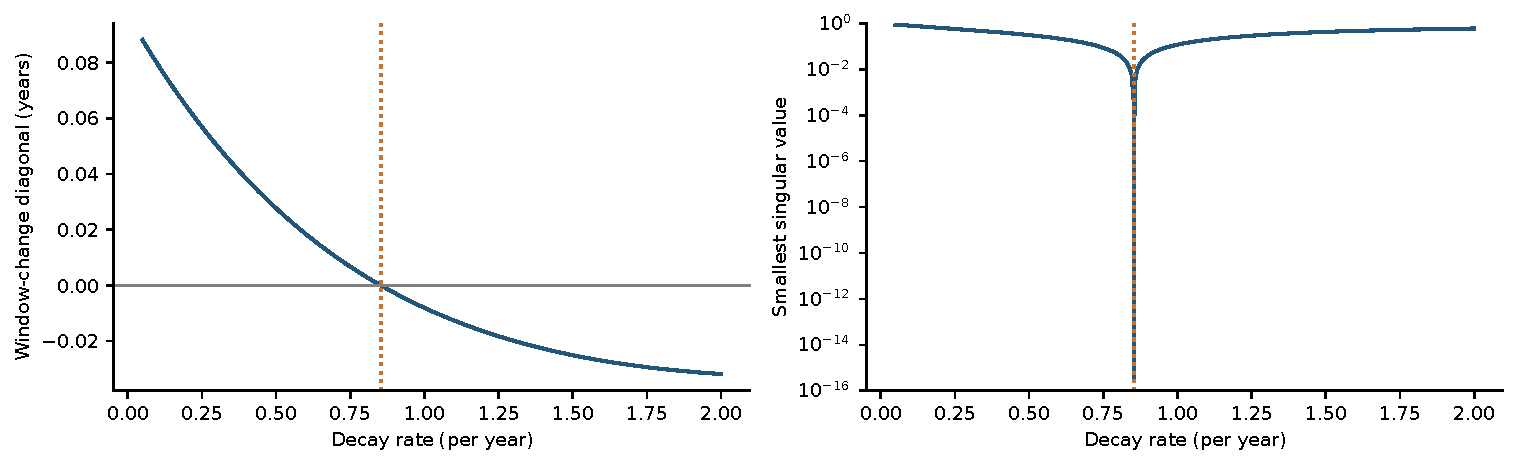
\includegraphics[width=.96\textwidth]{figures/critical_shape.pdf}
\caption{The same calendar can identify at one loading and fail at another. Left: either window-change diagonal in the eight-cell background matrix, in years. Right: smallest singular value of the meeting-free matrix after scaling each background column to unit Euclidean norm. The dotted line marks $\kappa^*$. The normalization removes arbitrary column units, not the loss of information.}\label{fig:criticalshape}
\end{figure}

\subsection{Futures means restore rank, but can add very little precision}
For the same ideal panel and parallel loadings, a calendar-quarter background has rank 23 of 24 columns, and a cell at every meeting has rank 24 of 33. Stacking the additional mean rows \eqref{eq:zrows} gives full column rank in both cases, and with a separate background rate in every expiry gap. These finite-matrix statements are reproduced in the accompanying calendar example.

An explicit confounding direction shows the scale of the extra information. Start with all meeting variances equal to $100$ bp$^2$ and background rates equal to $2500$ bp$^2$/year on the meeting-date partition. Increase the rate on 18 March--29 April 2026 by $360$ bp$^2$/year, and decrease the 18 March and 29 April meeting variances by $23$ and $19$ bp$^2$, respectively. Every option-variance row is unchanged: the affected cell contributes 23 days before the April expiry and 19 days in the next gap. Yet the mean adjustment $z$ changes by at most $1.86\times10^{-9}$ over the panel. For a quarterly future a 0.5 bp rate error changes $\log G_0$ by about $1.3\times10^{-5}$. Thus full rank of the richer observation matrix does not imply useful resolution at that precision. The calculation concerns the additional $z$ rows; known-curve $p$ rows are a further observation set.

\section{Additional results for the one-variance baseline}\label{app:baseline}
\subsection{What happens to the meeting-risk ranges?}
For dates that fit a stated tolerance, we solve the endpoint problems \eqref{eq:LP}. Figure~\ref{fig:empiricalranges} uses 18 June, the earliest sample date on which all three background specifications fit at 1 bp. Selecting it by this rule makes the example reproducible; it is not presented as a typical date.

For the 16 September meeting, constant background gives a range of $[689,1149]$ bp$^2$. With 90-day cells it is $[507,1407]$; with a separate rate in each expiry gap it is $[0,1450]$. For the 27 January 2027 meeting, the constant-background range is $[1870,2990]$ bp$^2$, whereas both flexible specifications permit zero. Thus a claim of strictly positive meeting risk can depend on the background restriction even when all specifications fit within the same price tolerance. For scale, the constant-background September range corresponds to a meeting standard deviation of approximately 26.2--33.9 bp; the expiry-gap range allows 0--38.1 bp.

The zero lower bounds with an expiry-gap background are structural: replacing each gap's event contribution by an equal amount of background variance leaves its observed increment unchanged. The data illustrate the size of the compatible ranges, not a newly discovered source of nonidentification.

The total variance of all eight meetings in this example is constrained to $[5308,6582]$ bp$^2$ under constant background, $[507,8892]$ with 90-day cells, and $[0,9376]$ with an expiry-gap background. Grouping meetings does not remove uncertainty about how much risk belongs to meetings at all. These are sharp conditional ranges for the diagnostic's interval observations; different coordinate endpoints need not occur at the same allocation.

\begin{figure}[ht]
\centering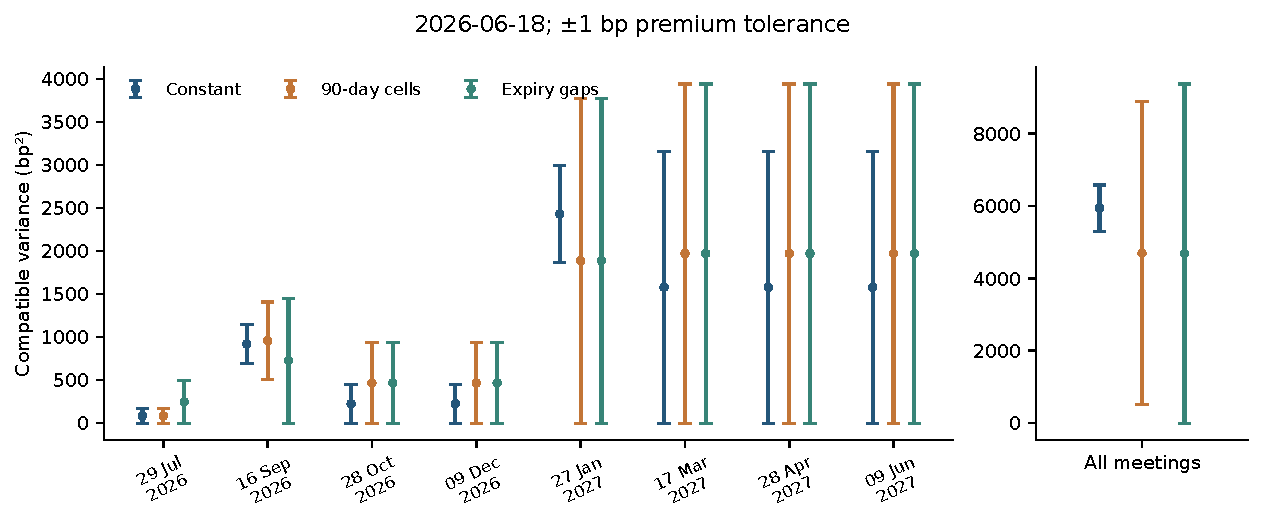
\includegraphics[width=\textwidth]{figures/empirical_ranges.pdf}
\caption{Compatible meeting variances in the normal diagnostic on 18 June 2026, using every selected strike within a 1 bp premium tolerance. Left: marginal ranges by meeting. Right: the jointly optimized total across meetings, on a separate vertical scale. All endpoints are shown without clipping; the individual and total panels have different scales. The markers are interval midpoints, not point estimates.}\label{fig:empiricalranges}
\end{figure}

\FloatBarrier
\subsection{Omitted-strike and omitted-expiry checks}
Figure~\ref{fig:empiricalchecks} collects the omitted-strike and same-expiry midcurve diagnostics. Two exercises check information outside a fitted input. First fit \eqref{eq:normalproxy} exactly to the closest out-of-the-money strike in each standard chain and price its other selected strikes. Across 555 chains, the median largest omitted-strike error is 1.000 bp and the maximum is 3.851 bp. Allowing the variance to fit all strikes helps: the median best possible uniform error within one chain is 0.747 bp. It still exceeds the tighter tolerance scenarios.

The second exercise withholds the entire second chronological expiry on each date. All remaining selected strikes constrain the constant-background model. The parameters and observation matrix retain the full meeting horizon, so removing the expiry does not silently remove an event parameter. At 0.5 bp, the training set is feasible on four dates; at 1 bp, on 26. On those dates, optimize the variance at the omitted expiry over all feasible allocations and convert its extrema to a premium range at the held-out chain's closest strike. Every held quote interval overlaps its prediction range. The median prediction width is 1.390 bp at the tighter tolerance and 3.253 bp at the wider one. This fixed screen produces no out-of-range candidate. The other dates fail at the training stage and supply no calibrated prediction interval.

This is a same-date omitted-contract check, not a forecast on a later date. It tests only the closest strike of the withheld chain; overlap there does not establish a fit to that chain's other strikes. The small feasible sample and the width of the ranges also prevent interpreting the absence of a candidate as evidence that the model is accurate or that the market offers no relative-value opportunities.


\begin{figure}[ht]
\centering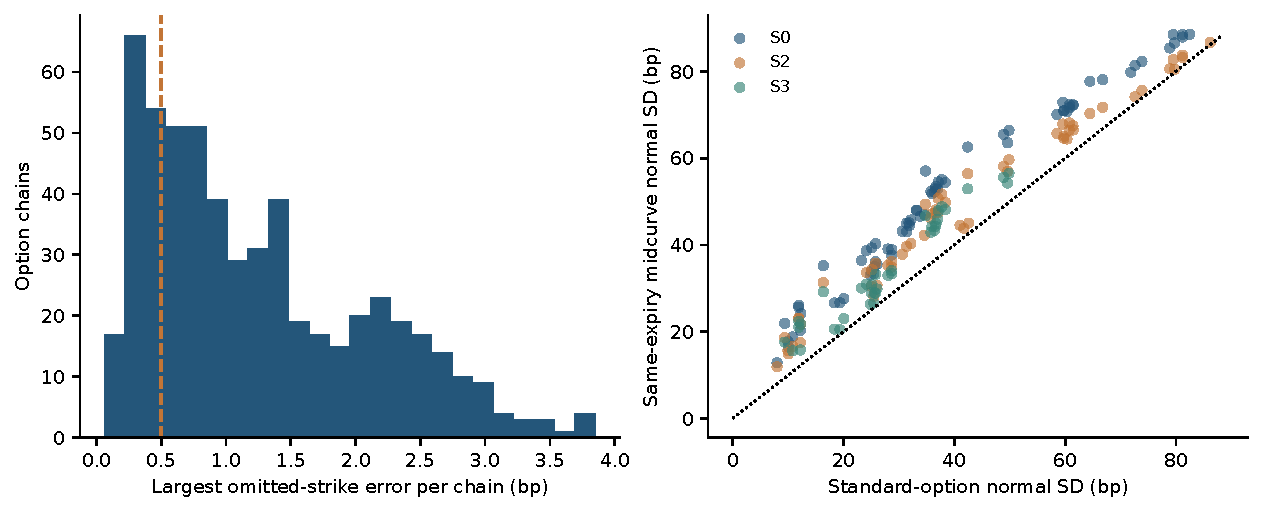
\includegraphics[width=\textwidth]{figures/empirical_price_checks.pdf}
\caption{Checks beyond a closest-strike fit. Left: largest error at omitted strikes in each standard chain; the dashed line is 0.5 bp. Right: normal standard deviations inferred separately from closest strikes in standard options and same-expiry midcurves. Equality is the parallel diagnostic's prediction. Differences can reflect maturity loadings, distributional shape, or exercise effects; this experiment does not identify their separate contributions.}\label{fig:empiricalchecks}
\end{figure}

\FloatBarrier

\section{Reproducibility, notation, and proof scope}\label{app:implementation}
The accompanying directory contains the LaTeX source, original data files, extracted panels, and offline Python programs. The example program reproduces the deterministic theoretical illustrations. The empirical program reproduces the historical-sample figures and calibration outputs using NumPy, SciPy, and Matplotlib. A separate decomposition program compares the saved independent-chain and calendar-fit errors. It performs monotone scalar inversion and linear programming, without simulating paths. The input hashes identify the exact versions of the three prepared datasets used in the analysis.

The synthetic example uses exact Gaussian cash prices. Its background volatility remains constant through the end of accrual. Discount factors and forward-measure means are fixed at their generating values. Its bounds are exact for the extracted variance observations; the additional structural restrictions tying those fixed means to candidate variances are not imposed. The empirical analysis uses the normal diagnostic \eqref{eq:normalproxy} and the smile-based ATM proxy \eqref{eq:smileatm}, with the selection rule and background schedules stated in Section~\ref{sec:empirical}. Puts and calls enter according to the selected out-of-the-money side; no European parity equation is imposed on the American settlements.

The data provenance records source locations, units, strike decoding, contract mappings, archive coverage, and missing inputs. Calendar ranks use only meetings after the valuation date and no later than the last retained expiry. The analysis is repeated separately by date; it imposes neither temporal smoothing nor a physical-measure time-series law. Market observations across dates share contracts and are not treated as independent statistical replications.

For the minimum-error calculation, all strike intervals at an expiry are intersected before the feasibility problem is solved. Bisection terminates when the premium-tolerance bracket is below 0.0001 bp. The code verifies price inversion, the linear constraints at both optimized endpoints, and price residuals at the reported feasible tolerance. The local calendar-hedge sensitivity is also checked by finite differences. Infeasible training sets do not generate prediction intervals. No held-out price is used to choose its training tolerance.

\subsection{Smile, loading, and exercise calculations}\label{app:empiricalmethod}
The extension program fits the mixture \eqref{eq:mixture} separately by chain. To scale the optimization, divide displacements and standard deviations by the closest-strike implied normal standard deviation, floored at 1 bp. In these units constrain $d\in[-2,2]$ and $\log s_j\in[-3,1.5]$. Use starts $(0,0,0)$, $(0.5,-0.5,0.2)$, and $(-0.5,-0.5,0.2)$ for $(d,\log s_1,\log s_2)$, retaining the converged solution with smallest squared price residual. All 555 standard fits converge. These bounds and local optimization are part of the interpolation specification; global optimality or identification of mixture parameters is not asserted. The omitted-closest-strike calculation uses the same starts and bounds and never fits to the withheld premium. Its scale uses only training strikes.

The loading calculation integrates the maturity average analytically and uses 20-point Gauss--Legendre quadrature in shock time, separately on each background cell. For every candidate shape, weighted nonnegative least squares gives the date-specific allocation. The original 37-shape grid includes the parallel case $\chi=0$. The free-long-end grid uses
\begin{align*}
\kappa&\in\{0.25,0.5,0.75,1,1.25,1.5,2,3,4\},\\
\chi_1&\in\{0,0.5,1,2,4,8,12,16\},\qquad
\chi_2\in\{0,0.25,0.5,1,2,4,8\}.
\end{align*}
Removing eight duplicates of the parallel shape leaves 496 shapes. Its pure-hump subset has 64 distinct shapes. When the selected amplitude reaches a grid boundary, the sensitivity grid uses both amplitudes in $\{0,1,2,4,8,12,16,24,32,48,64\}$ and the same decay grid: 1,081 distinct shapes. This is a discrete grid check, not a continuous global optimum or parameter confidence region. Shape selection and date-specific fitting exclude all S3 observations in both searches. The additional family itself was chosen after the original S3 failure, so that comparison reuses an examined sample. The subsequent all-product interval analysis is separate; its fit counts and ranges are not held-out results. Shape-profile endpoints are the smallest lower and largest upper endpoints across feasible shapes on the original grid.

The American tree uses increments $-\sqrt{3\cV_{\rm ATM}/n}$, $0$, and $+\sqrt{3\cV_{\rm ATM}/n}$ with probabilities $1/6$, $2/3$, and $1/6$. Each step discounts by $D^{1/n}$. Backward induction takes the maximum of discounted continuation and intrinsic value for the American claim, and continuation alone for the European claim. Their difference on the same grid isolates exercise value. At zero discount rate the code checks that the exercise premium vanishes. The European price is also compared with the analytic normal formula. This benchmark holds the normal variance rate and discount rate constant and does not model scheduled jumps.

For the empirical proxies, uncertainty about smile interpolation, exercise, the forward-measure mean, and the loading shape is not combined into a statistical confidence set. The reported intervals answer explicit sensitivity questions conditional on those choices. A listed-contract structural estimation would require a joint smile and exercise model, the appropriate stochastic discounting, and a convention-matched independent curve. Neither the mixture fit nor its good local interpolation test supplies those additional ingredients.

\subsection{Conditional ranges under the original hump}\label{app:shapeprofile}
Using all 256 standard and same-expiry midcurve ATM observations gives feasible sets conditional on the original hump $(\chi,\kappa)=(4,0.75)$. The median minimum ATM-price allowance drops from 3.319 bp under parallel loading to 1.136 bp with the hump and constant background, 1.078 bp with 90-day cells, and 0.936 bp with expiry-gap cells. At a 1 bp allowance, these three humped specifications fit respectively 2, 5, and 9 of the fourteen dates; no parallel specification fits a date.

On 22 July, the first date fitting all three humped backgrounds at that allowance, the September-meeting ranges are $[88,550]$, $[0,550]$, and $[0,1038]$ bp$^2$ for constant, 90-day, and gap backgrounds. The January 2027 ranges are $[414,973]$, $[378,2113]$, and $[314,2514]$ bp$^2$. Same-expiry windows now add background information: with expiry-gap cells the matrix rank rises from 7 under parallel loading to 12 out of 15 columns under the hump. In contrast to the standard-only parallel experiment, assigning each increment to its own background cell no longer makes all meeting lower bounds vanish.

Conditioning on an estimated shape can overstate this information. Taking the union of the constant-background feasible sets over the entire grid gives September range $[0,550]$ and January range $[0.16,973]$ bp$^2$ on 22 July. Only two grid shapes fit that date within 1 bp. The tiny positive January endpoint is specific to the finite grid; it is not a positive bound over all smooth loadings. These original-hump calculations illustrate the effect of conditioning on a shape. They are separate from the free-long-end prediction comparison in Section~\ref{sec:humpfit}.


\subsection{Exact ATM calculation for discrete meetings}\label{app:additivity}
This synthetic example isolates the observation transform. It specifies an arithmetic futures martingale directly, rather than claiming that binary jumps satisfy the Gaussian rate model. Let meetings occur at $T_i=i/8$ year, let $\epsilon_i$ be independent symmetric signs, and let $W$ be an independent Brownian motion. At expiry $S_n=n/8$, put
\[
X_n=25\sum_{i=1}^n\epsilon_i+\sigma W_{S_n},\qquad
D_n=e^{-0.04S_n},\qquad n=1,\ldots,8.
\]
Displacements are in bp and $\sigma$ in bp per square-root year. Its true variance is $625n+\sigma^2S_n$. Conditional on $k$ positive outcomes, the displacement is normal with mean $\mu_{nk}=25(2k-n)$ and standard deviation $s_n=\sigma\sqrt{S_n}$. Thus its exact European ATM price is
\[
\frac{C_n}{D_n}=2^{-n}\sum_{k=0}^n\binom nk
 \left[\mu_{nk}\Phi(\mu_{nk}/s_n)+s_n\varphi(\mu_{nk}/s_n)\right],
\]
using $(\mu_{nk})^+$ when $s_n=0$. Define $\cV_{{\rm ATM},n}=2\pi(C_n/D_n)^2$ and $\cV_{{\rm ATM},0}=0$.

The increments are independent and identically distributed, so additivity of the proxy would imply $\cV_{{\rm ATM},n}=n\cV_{{\rm ATM},1}$. The resulting ATM-price error is
\[
D_n\sqrt{n\cV_{{\rm ATM},1}/(2\pi)}-C_n.
\]
Alternatively, an unconstrained meeting-by-meeting fit with the correct background variance rate would infer
\[
\widehat v_n=\cV_{{\rm ATM},n}-\cV_{{\rm ATM},n-1}-\sigma^2/8.
\]
All these increments are nonnegative in the four computed scenarios, so an exact nonnegative calendar fit is possible. Yet $\widehat v_n$ need not be 625 bp$^2$.

\begin{center}\small
\begin{tabular}{rrr}
\toprule
$\sigma$ (bp/$\sqrt{\mathrm{year}}$) & Maximum price error (bp) & Range of $\widehat v_n$ (bp$^2$)\\
\midrule
0 & 7.697 & $[0,1246.4]$\\
25 & 5.005 & $[351.6,904.6]$\\
50 & 2.323 & $[549.3,770.4]$\\
100 & 0.532 & $[616.6,672.3]$\\
\bottomrule
\end{tabular}
\end{center}
Figure~\ref{fig:additivity} displays the errors and two allocation examples. Even the largest background in the table leaves a maximum price error above 0.25 bp. In the Gaussian control, replacing each sign jump by an independent centred normal variable of variance 625 makes the ATM proxy equal the true variance at every expiry; both errors then vanish. The discrete example demonstrates a possible structural error, not its empirical size in the settlement panel.

\begin{figure}[ht]
\centering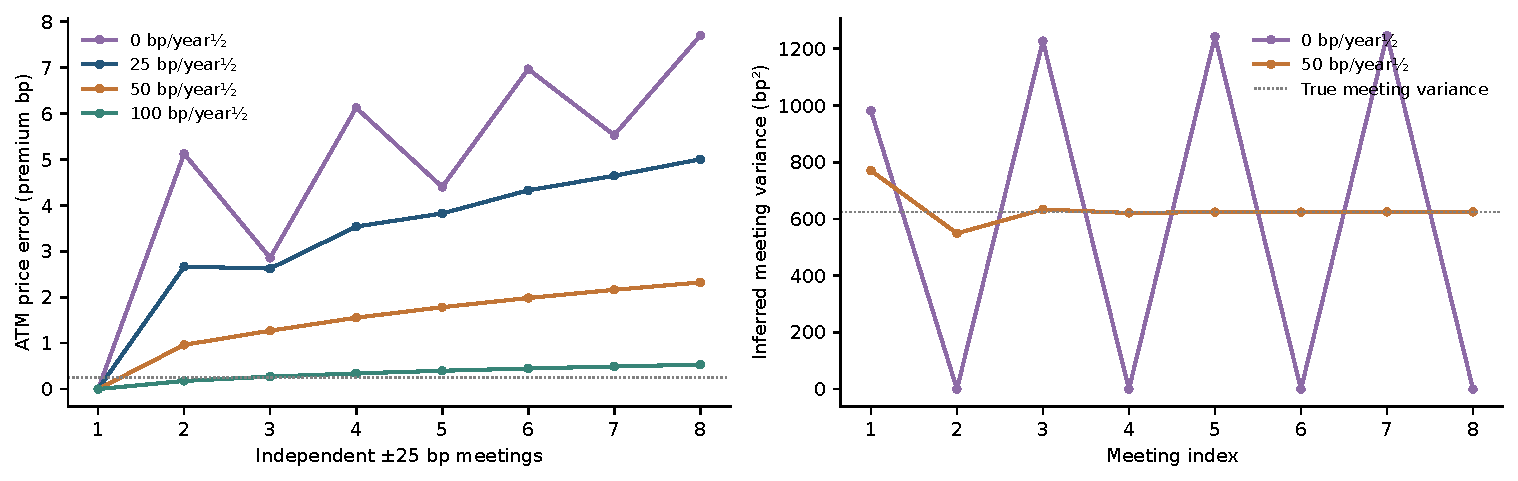
\includegraphics[width=\textwidth]{figures/atm_additivity.pdf}
\caption{Independent $\pm25$ bp meetings with Gaussian background. Left: ATM-price error from adding the identical one-increment ATM proxies; the dotted line is 0.25 bp. Right: meeting variances inferred by fitting each expiry exactly and subtracting the known background. Every actual meeting has variance 625 bp$^2$ (dotted line).}\label{fig:additivity}
\end{figure}

\FloatBarrier
\subsection{Second-moment and front-loading sensitivities}\label{app:finalsensitivities}
\paragraph{Second moments.}
The fitted mixture has mean zero and variance
$\widehat{\cV}_{2,\ell}=d_\ell^2+(s_{1,\ell}^2+s_{2,\ell}^2)/2$.
Unlike the ATM proxy, this is the variance of the fitted law. Its use still extrapolates that law beyond the observed strikes, and fitting separate expiry laws does not establish independent increments or a common pricing measure. We apply the parallel calendar equation to these moments as a companion sensitivity calculation.

For comparability, retain the numerical ATM-price allowances $\varepsilon_\ell$ in \eqref{eq:robustallowance}. Multiplying the entire centred mixture displacement by a positive scalar multiplies its ATM price by that scalar and its second moment by its square. Thus an ATM-scale perturbation induces a moment interval. Widen that interval by an additional relative allowance $\zeta\in\{0,0.10,0.25,0.50\}$:
\begin{equation}\label{eq:momentinterval}
(1-\zeta)\widehat{\cV}_{2,\ell}
 \left\{\left(1-\frac{\varepsilon_\ell}{\widehat c_{{\rm ATM},\ell}}\right)^+\right\}^2
\ \leq\ (\mathsf A\theta)_\ell\ \leq\
(1+\zeta)\widehat{\cV}_{2,\ell}
 \left(1+\frac{\varepsilon_\ell}{\widehat c_{{\rm ATM},\ell}}\right)^2.
\end{equation}
The values of $\zeta$ are sensitivity scenarios, not estimated tail-error bounds or confidence levels. The numerical $\varepsilon_\ell$ are reused as scale allowances; their exercise and mean components are not recalculated under the mixture law. This experiment does not transfer the Gaussian seed-containment argument to a different pricing model.

On 18 June the ratio $\widehat{\cV}_{2,\ell}/\widehat{\cV}_{{\rm ATM},\ell}$ ranges from 0.892 to 1.392 across seven expiries. With $\zeta=0$, constant and 90-day backgrounds are infeasible; expiry-gap background is feasible and permits zero for both headline meetings. Table~\ref{tab:momentcheck} reports the wider scenarios. At $\zeta=0.50$, all three specifications permit zero for both meetings. The positive constant-background bounds at $\zeta=0.10$ therefore demonstrate a conditional contrast between backgrounds, not distribution-free positive lower bounds.

\begin{table}[ht]
\centering\small
\begin{tabular}{rlrr}
\toprule
Extra allowance & Background & 16 September 2026 & 27 January 2027\\
\midrule
10\% & Constant & $[275,1058]$ & $[1549,4229]$\\
 & 90-day cells & $[0,1343]$ & $[0,5125]$\\
 & Each expiry gap & $[0,1470]$ & $[0,5125]$\\
25\% & Constant & $[0,1552]$ & $[91,5740]$\\
 & 90-day cells & $[0,1789]$ & $[0,6487]$\\
 & Each expiry gap & $[0,1895]$ & $[0,6487]$\\
\bottomrule
\end{tabular}
\caption{Mixture-second-moment meeting-variance ranges on 18 June under \eqref{eq:momentinterval}, in bp$^2$, rounded to the nearest integer. These are sensitivity ranges for an extrapolated second moment.}\label{tab:momentcheck}
\end{table}

\paragraph{Flattening the front of the loading.}
Write the selected free-level loading as a function of maturity distance,
$\phi(\tau)=1+18\tau e^{-1.5\tau}+8(1-e^{-1.5\tau})$.
For a cutoff $h\geq0$, replace it by $\phi(\max\{\tau,h\})$ and divide by its value at $\tau=1$. This keeps the tail unchanged up to a common scale and makes the front constant. We rebuild the 22 July all-product exposure matrix with expiry-gap background cells; there are 17 observations and 15 parameter columns. No coefficients are refitted. Maturity averaging is analytic, and shock-time integration is split where a window crosses the cutoff.

The ranks for $h=0,0.5,1,1.5$ years are all 12. In the same ACT/360 parameter coordinates, the smallest nonzero singular value divided by the largest is respectively $4.05\times10^{-4}$, $7.64\times10^{-5}$, $7.14\times10^{-5}$, and $1.51\times10^{-6}$. Removing the first half-year's slope weakens this relative sensitivity by a factor of 5.3 without destroying exact rank. Setting $h=4$ years flattens the entire observed exposure domain, reproduces the parallel matrix, and reduces rank to 7. The rank increase therefore does not depend exclusively on the steep front, but its numerical strength is sensitive to that part of the curve. These singular values compare the stated coordinate scaling; they are not invariant measures of statistical precision.\FloatBarrier

\subsection{Proof scope and notation}
The arguments in Appendix~\ref{app:pricing} use standard Brownian integration, stochastic Fubini for bounded deterministic integrands, and elementary Gaussian conditioning. They assume a probability space carrying the independent Brownian motion and Gaussian meeting variables specified in Section~\ref{sec:prices}. The rank, interval, and polytope arguments are finite-dimensional results independent of a stochastic-calculus construction.

The mathematical arguments are supplied in this manuscript. The accompanying source map identifies the corresponding Lean statements and their explicit hypotheses; it also distinguishes the general American stopping argument and Corollary~\ref{cor:generalaggregate}, which are proved here, from the narrower formalized statements. The numerical analysis is separate from those formal proofs.

\begin{longtable}{p{.19\textwidth}p{.72\textwidth}}
\caption{Notation used in the main results.}\label{tab:notation}\\
\toprule Symbol & Meaning\\\midrule\endfirsthead
\toprule Symbol & Meaning\\\midrule\endhead
$t,T,H,T_n$ & Observation time, maturity, finite horizon, and meeting dates.\\
$Q,\F_t,W$ & Pricing measure, information at $t$, and Brownian driver.\\
$X_n,v_n,\xi_n(T)$ & Announcement level, its variance, and the full forward-curve announcement change.\\
$f_0(T),f(t,T)$ & Initial and time-$t$ instantaneous forward rates for maturity $T$.\\
$\alpha(t,T),\sigma(t,T)$ & Forward drift and Brownian sensitivity in the general model.\\
$\sigma(s),u_j,n_b$ & Continuous volatility; its squared value on background cell $j$; number of cells.\\
$r_t,B_t,P(t,T)$ & Short rate, bank account, and zero-coupon bond price.\\
$S,[a,b],\delta$ & Option expiry, futures accrual window, and window length $b-a$.\\
$R,G_t,F_t$ & Accrual accumulation, its conditional expectation, and futures rate $(G_t-1)/\delta$.\\
$D,m,q$ & Discount factor $P(0,S)$, option forward-measure mean, and log variance.\\
$p,z$ & Futures convexity exponent and the mean adjustment $\log G_0-\log m$.\\
$\cV(S)$ & Accumulated rate variance; $q/\delta^2$ before accrual in the parallel model.\\
$\cV_{\mathrm N},\theta_{\mathrm N}$ & Variance and meeting/background parameters of the separate empirical normal diagnostic.\\
$\widehat{\cV}_{\rm ATM},\widehat c_{\rm ATM},\theta_{\rm ATM}$ & Mixture-interpolated ATM normal variance, its ATM premium, and the parameters of its additive working schedule.\\
$\widehat{\cV}_{2,\ell},\zeta$ & Fitted mixture second moment and additional relative moment allowance in Appendix~\ref{app:finalsensitivities}.\\
$\chi,\kappa$ in \eqref{eq:humpshape} & Hump amplitude and loading decay; $\chi_1,\chi_2$ in \eqref{eq:levelshape} allow a separate long-end level.\\
$\mathcal I$ & Inverse of the fixed-mean at-the-money cash-price formula.\\
$\theta,\mathsf A$ & Nonnegative variance parameters and variance observation matrix.\\
$E,\Lambda_E$ & Indices of meeting-free expiry gaps and their background exposure matrix.\\
$\phi,\beta_\ell,\mathsf D_{\ell j}$ & Known maturity shape, its average over window $\ell$, and weighted background exposure.\\
$V,M_1;V_A,M_{1,A}$ & Pre-cutoff meeting totals and date-weighted totals; their extensions including continuous variance.\\
$\Theta,\Pi(V,M_1)$ & Price-tolerance feasible set and exact aggregate-compatible polytope.\\
$\boldsymbol V(t)$ & Vector of conditional short-rate jump variances in the factor model.\\
$\mathsf K,\eta$ & Deterministic scale-exposure matrix and its nonnegative interval weights.\\
$Z_j,\vartheta_j,\alpha_j,\rho_j$ & Square-root variance state, mean-reversion speed, volatility of volatility, and leverage correlation.\\
$\mathsf L,\boldsymbol c,J,\ell$ & Stochastic variance loading matrix, deterministic offset, active factor set, and support endpoints.\\
\bottomrule
\end{longtable}

\bibliographystyle{plainnat}
\bibliography{refs}
\end{document}
